\documentclass{article}

% ready for submission
\usepackage[final]{neurips_2023}

\usepackage[utf8]{inputenc} % allow utf-8 input
\usepackage[T1]{fontenc}    % use 8-bit T1 fonts
\usepackage{hyperref}       % hyperlinks
\usepackage{url}            % simple URL typesetting
\usepackage{booktabs}       % professional-quality tables
\usepackage{amsfonts}       % blackboard math symbols
\usepackage{nicefrac}       % compact symbols for 1/2, etc.
\usepackage{microtype}      % microtypography
\usepackage{xcolor}         % colors
\usepackage{graphicx}       % For adding figures/spectrograms

\title{Task 3: Data Exploration Report}

\author{% 
   Validated Encoders \AND
  Amr ABDULLAH
  \And
  Ibrahim MUHAMMAD
}

\begin{document}

\maketitle

\section{Verify Annotations \& Qualitative Analysis}
We reviewed 10 audio recordings via Label Studio. For each recording, we compared annotations from multiple annotators, checked class assignments against class definitions, verified temporal precision of onsets and offsets, ensured the one-second rule was respected for pauses, and identified any missed events. Incorrect annotations were corrected where possible and ambiguous cases were commented and accepted.

\subsection{Summary of Disagreements}
% Detail the kinds of disagreements and rule violations you observed during your Label Studio reviews.
% Does disagreement always imply that at least one annotator violated the rules?
The overall disagreement was mainly about temporal boundaries, specifically onsets and offsets. In many cases the one-second rule was violated, and in some cases target classes audible in the recording were neither annotated nor stated in the metadata. Disagreement does not always imply that annotators explicitly violated the rules. Short or faintly audible sounds, critical overlapping among events, and transitions between similar sources (e.g., toilet refilling and running water) were the most frequent causes of disagreement among annotators.

\subsection{Case Study}
% Present ONE clear case of a rule violation or a significant disagreement.
% Include the filename, a visualization (like a spectrogram), a textual description, and your interpretation.
Audio file 003679 lists \textit{phone\_ringing} and \textit{light\_switch} as target classes. Upon review, clearly audible footsteps are present throughout the recording but are neither mentioned in the metadata nor annotated by one of the annotator. Furthermore, the two annotators disagree on the \textit{phone\_ringing} boundaries: one annotator clearly violates the one-second rule by not splitting a phone ringing event that contains a pause longer than one second. Figure~\ref{fig:casestudy} shows the side-by-side comparison.

\section{Annotations}

\subsection{Annotator Agreement}
% Explain how you quantified agreement and present the general and class-wise estimates.
% Do the temporal annotations agree with the user-specified target class tags?
We quantified agreement using Cohen's Kappa and Jaccard similarity, computed pairwise across all annotator pairs in files with at least two annotators. Per-class kappa was computed only in files where at least one annotator marked the class as present, avoiding inflated scores from trivial zeroes agreements.

The overall mean Cohen's Kappa across 5,735 pairs is $\kappa = 0.788$ (std: 0.201), indicating \textbf{substantial agreement} on the Landis \& Koch scale. All 15 classes achieve at least substantial agreement. The lowest agreement is for \textit{footsteps} ($\kappa = 0.770$), \textit{door\_open\_close} ($\kappa = 0.839$), and \textit{light\_switch} ($\kappa = 0.898$)---short events with ambiguous temporal boundaries. The highest agreement is for \textit{coffee\_machine} ($\kappa = 0.983$), \textit{vacuum\_cleaner} ($\kappa = 0.981$), and \textit{bell\_ringing} ($\kappa = 0.979$)---sustained, acoustically distinct sounds (see Figure~\ref{fig:agreement}).

The mean overlap ratio between annotated classes and the uploader's target class tags is 0.90. In 85.6\% of files all target classes appear in the annotations, confirming that temporal annotations generally agree with uploader metadata. In 16.6\% of files annotators identified additional classes beyond the targets, probably detected as incidental background events.

Pairs involving the recording owner show slightly higher agreement ($\kappa = 0.792$, $n = 4{,}170$) than pairs without ($\kappa = 0.776$, $n = 1{,}565$), suggesting first-hand knowledge of the recorded scene which provides a slight annotation advantage.


\subsection{Convert Annotations to Labels}
% Describe how you aggregated the [T, C, A] annotations into binary prediction targets.
% Discuss the assumptions your method relies on and under what conditions the labels could be incorrect.

We convert the raw annotation array $[T, C, A]$ into binary labels $[T, C]$ in two steps. First, each annotator's soft overlap value is binarized at threshold of 0.5: values above indicate the event is present. Second, we take the majority vote by averaging binary decisions across annotators and thresholding at $\geq 0.5$.

This assumes all annotators are equally reliable and that overlap $>0.5$ constitutes presence. With two annotators (the most common case), a tie resolves as positive, introducing a slight bias toward labeling events as present. If all annotators make the same error, majority vote preserves it. Partial overlaps near 0.5 are sensitive to the exact threshold choice, e.g, 0.49 are not considered. 

\subsection{Label Characteristics}
% Describe the label characteristics (e.g., class frequency, average duration, co-occurrences).
The dataset spans 168,239 segments ($\sim$46.7 hours). The most frequent class is \textit{footsteps} (1,815 files, 15.3\% of total time); the rarest is \textit{bell\_ringing } (276 files, 1.5\%), revealing a significant class imbalance (see Table~\ref{tab:labels} and Figure~\ref{fig:labelfreq}).

Event durations vary by class type: sustained sounds have long durations (\textit{vacuum\_cleaner}: median 32s, \textit{microwave}: 24s, \textit{coffee\_machine}: 19s), while transient events are short (\textit{light\_switch}: 2s, \textit{door\_open\_close}: 3s). Approximately 7.3\% of segments are silent where no active classes are found (silent or non target classes). \textit{Footsteps} co-occur frequently with many other classes as expected.

 
\section{Audio Features}

\subsection{Metadata Distribution}
% Provide statistics or a visualization regarding recording properties like placement, devices, or locations.
Recording properties were extracted from the *.npz files. 53.9\% of device placement are static and 46.1\% mobile. The most common recording devices are smartphones (mainly iPhones). The most frequent recording environments are \textit{kitchen}, \textit{living room}, and \textit{office}, with strong environment-class coupling: kitchen recordings are dominated by \textit{running\_water} and \textit{cutlery\_dishes}, while office recordings feature \textit{keyboard\_typing} and \textit{phone\_ringing}.

\subsection{Feature Statistics}
% Summarize the basic statistics (mean, std, range) of the audio features.
The dataset contains 960 feature dimensions (14 base features $\times$ 4 aggregation methods). Feature scales vary dramatically: \textit{power\_max} reaches 67,941 while \textit{flatness} stays in $[0, 1]$, confirming that standardization is essential before any distance based method.

Temporal derivative features (\textit{mfcc\_d\_mean}, \textit{mfcc\_d2\_mean}) have means values ranging near zero across all classes. Their \textit{std} and \textit{min/max} aggregations do not carry useful information. Energy and power are not normally distributed (mean $\ll$ max), explained by probable outliers or burst events (non target classes) which can be considered as bias. 

\subsection{Feature Correlation}
% Explain your correlation analysis method. Which features (e.g., MFCCs and Mel-Spectrogram) are correlated?
% Include a visualization of the results.
We analyzed inter-group correlation using Pearson correlation on mean aggregated values. Strong correlations reflect known physical relationships: \textit{zcr}--\textit{centroid} ($r = 0.95$), \textit{rolloff\_high}--\textit{bandwidth} ($r = 0.96$), \textit{energy}--\textit{flux} ($r = 0.93$). MFCCs and mel spectrogram correlate at $r = 0.82$. Temporal derivatives (\textit{mfcc\_d}, \textit{mfcc\_d2}) show near-zero correlation with all other features ($|r| < 0.14$).

The class-wise feature profile (Figure~\ref{fig:profiles}) reveals distinctive acoustic fingerprints. \textit{Vacuum\_cleaner} shows the highest energy (+1.77$\sigma$) and mel spectrogram (+1.35$\sigma$), reflecting loud broadband noise. \textit{Running\_water} has the highest zcr (+1.41$\sigma$) and flatness (+1.20$\sigma$). \textit{Microwave} shows very low centroid ($-1.02\sigma$) and bandwidth ($-1.24\sigma$), for its low frequency nature and influnced by the buttons/ stat/end beeps. \textit{Footsteps} and \textit{keyboard\_typing} share similar, below average profiles, that make them difficult to separate.

\section{Feature Space Visualization}
We selected spectral features (mel spectrogram, centroid, bandwidth, flatness, contrast, rolloff) with mean and std aggregations (280 dimensions), chosen based on our correlation analysis for complementary spectral coverage with minimal redundancy. PCA compresses these to 50 components retaining 97.8\% of variance (only 9 components needed for 90\%), substantially outperforming alternative feature subsets we tested.

We filtered for single class segments with $\geq$80\% annotator agreement (76,716 segments), then subsampled 14,994 for t-SNE (perplexity=30, PCA initialization, 1,000 iterations). This achieved the lowest KL divergence (1.99) among all tested configurations. Figure~\ref{fig:tsne} shows well and clearly separated clusters for sustained sounds (\textit{vacuum\_cleaner}, \textit{running\_water}) and more diffuse, overlapping distributions for transient events (\textit{footsteps}, \textit{light\_switch}). Pairwise analysis confirms partial overlap between \textit{running\_water} and \textit{toilet\_flushing}, while \textit{vacuum\_cleaner} and \textit{microwave} form distinct clusters despite both being sustained appliance sounds.

\section{Conclusions}
% Give at least three examples of biases introduced during data collection/annotation and their potential consequences.

\subsection{Biases}
Three key biases were identified: (1)~\textbf{Device bias}---a small number of smartphone models dominate the dataset, introducing device specific frequency responses and noise floors that classifiers may learn instead of sound event characteristics. (2)~\textbf{Environment bias}---certain classes are strongly tied to specific rooms (e.g., \textit{running\_water} to kitchens), so a classifier may learn room acoustics rather than the sound event itself. (3)~\textbf{Annotator bias}---with mostly two annotators per file, systematic errors directly affect labels; the recording owner annotates with slightly higher agreement and may introduce bias toward intended target sounds.

\subsection{Dataset Suitability}
% Is the dataset suitable for training sound event detectors?
% What specific aspects will make learning a reliable classifier challenging?
The dataset is suitable for training sound event detectors, but several challenges exist. Class imbalance (\textit{footsteps} appears in $9\times$ more files than \textit{coffee\_machine}) requires handling. Similar class pairs (\textit{footsteps} vs.\ \textit{keyboard\_typing}, \textit{door} vs.\ \textit{wardrobe}) share overlapping feature profiles, making precise discrimination challenging. Feature scale differences require normalization. The high annotator agreement ($\kappa = 0.79$) provides generally reliable labels, though transient events may introduce label noise near temporal boundaries.

\subsection{Broader Impact}
% Discuss the positive and negative societal impacts of making this dataset public.
% Outline potential misuse scenarios and measures to promote ethical use.
A domestic sound dataset has many applications in areas such as elderly monitoring and smart home automation. However, it also presents risks of misuse, including unauthorized surveillance. To mitigate these concerns, dataset creators should ensure the anonymity of data contributors, limit redistribution and usage, and enforce strict ethical guidelines and agreements. Additionally, the dataset license should explicitly prohibit any use for surveillance purposes.

\clearpage
\section{Figures and Tables}


\subsection{Figures}
 
\begin{figure}[!h]
  \centering
  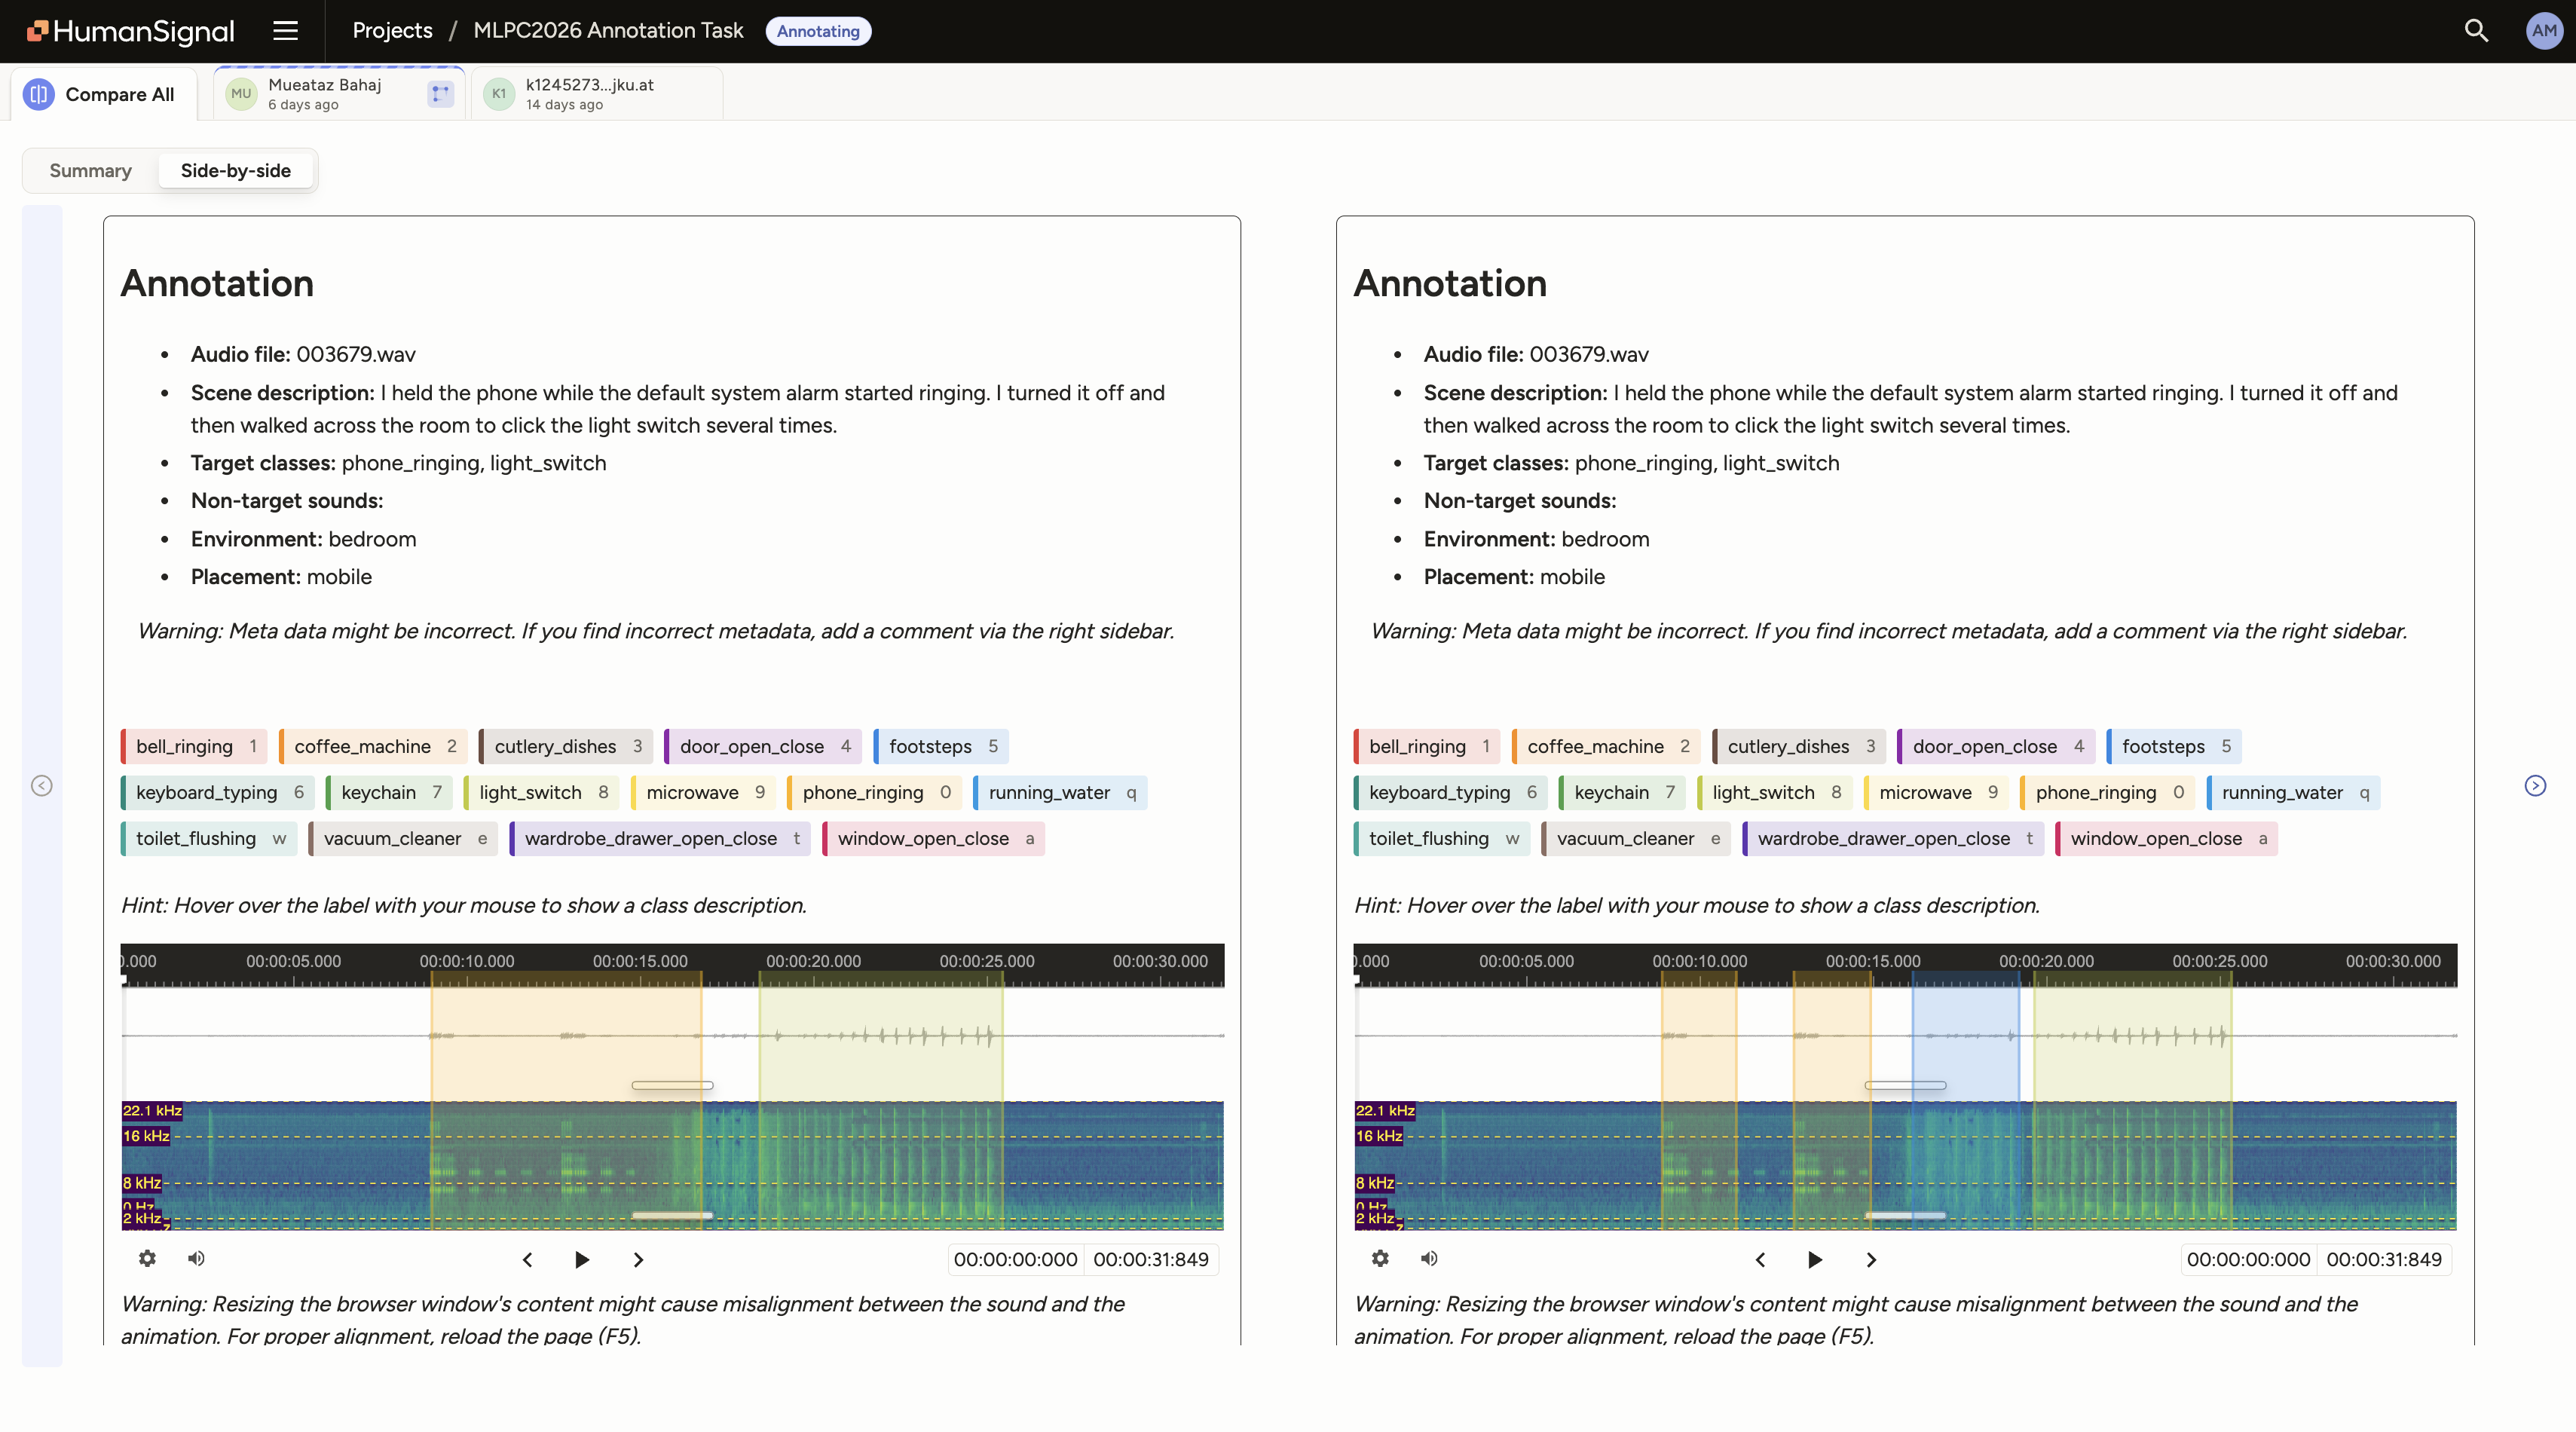
\includegraphics[width=\textwidth]{casestudy_003679.png}
  \caption{Side-by-side annotation comparison for file 003679. Annotator~1 (left) does not split the phone ringing region despite a pause exceeding one second. Also Footsteps are absent from the annotation.}
  \label{fig:casestudy}
\end{figure}

 
\begin{figure}[!h]
  \centering
  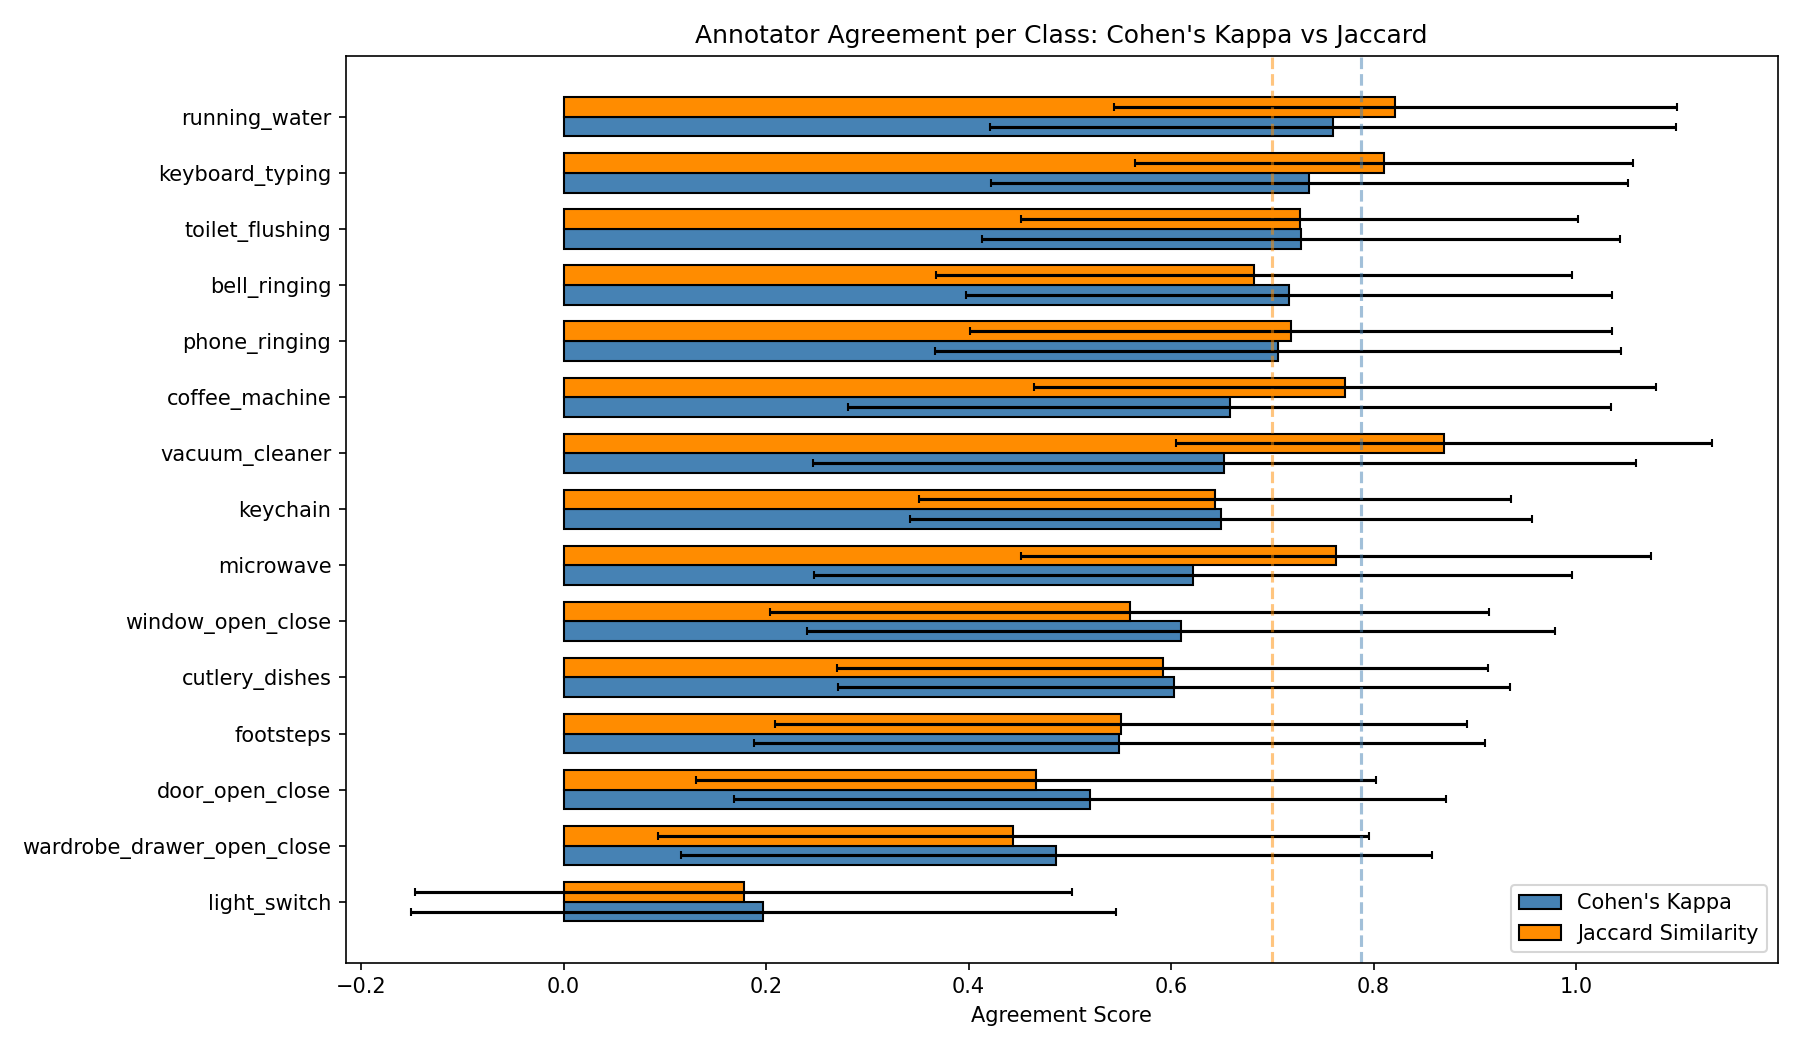
\includegraphics[width=\textwidth]{agreement_kappa_vs_jaccard.png}
  \caption{Class-wise annotator agreement: Cohen's Kappa vs.\ Jaccard similarity. Dashed lines indicate overall means. Transient events (footsteps, door) show lower agreement than sustained sounds (vacuum, coffee machine).}
  \label{fig:agreement}
\end{figure}

\begin{figure}[!h]
  \centering
  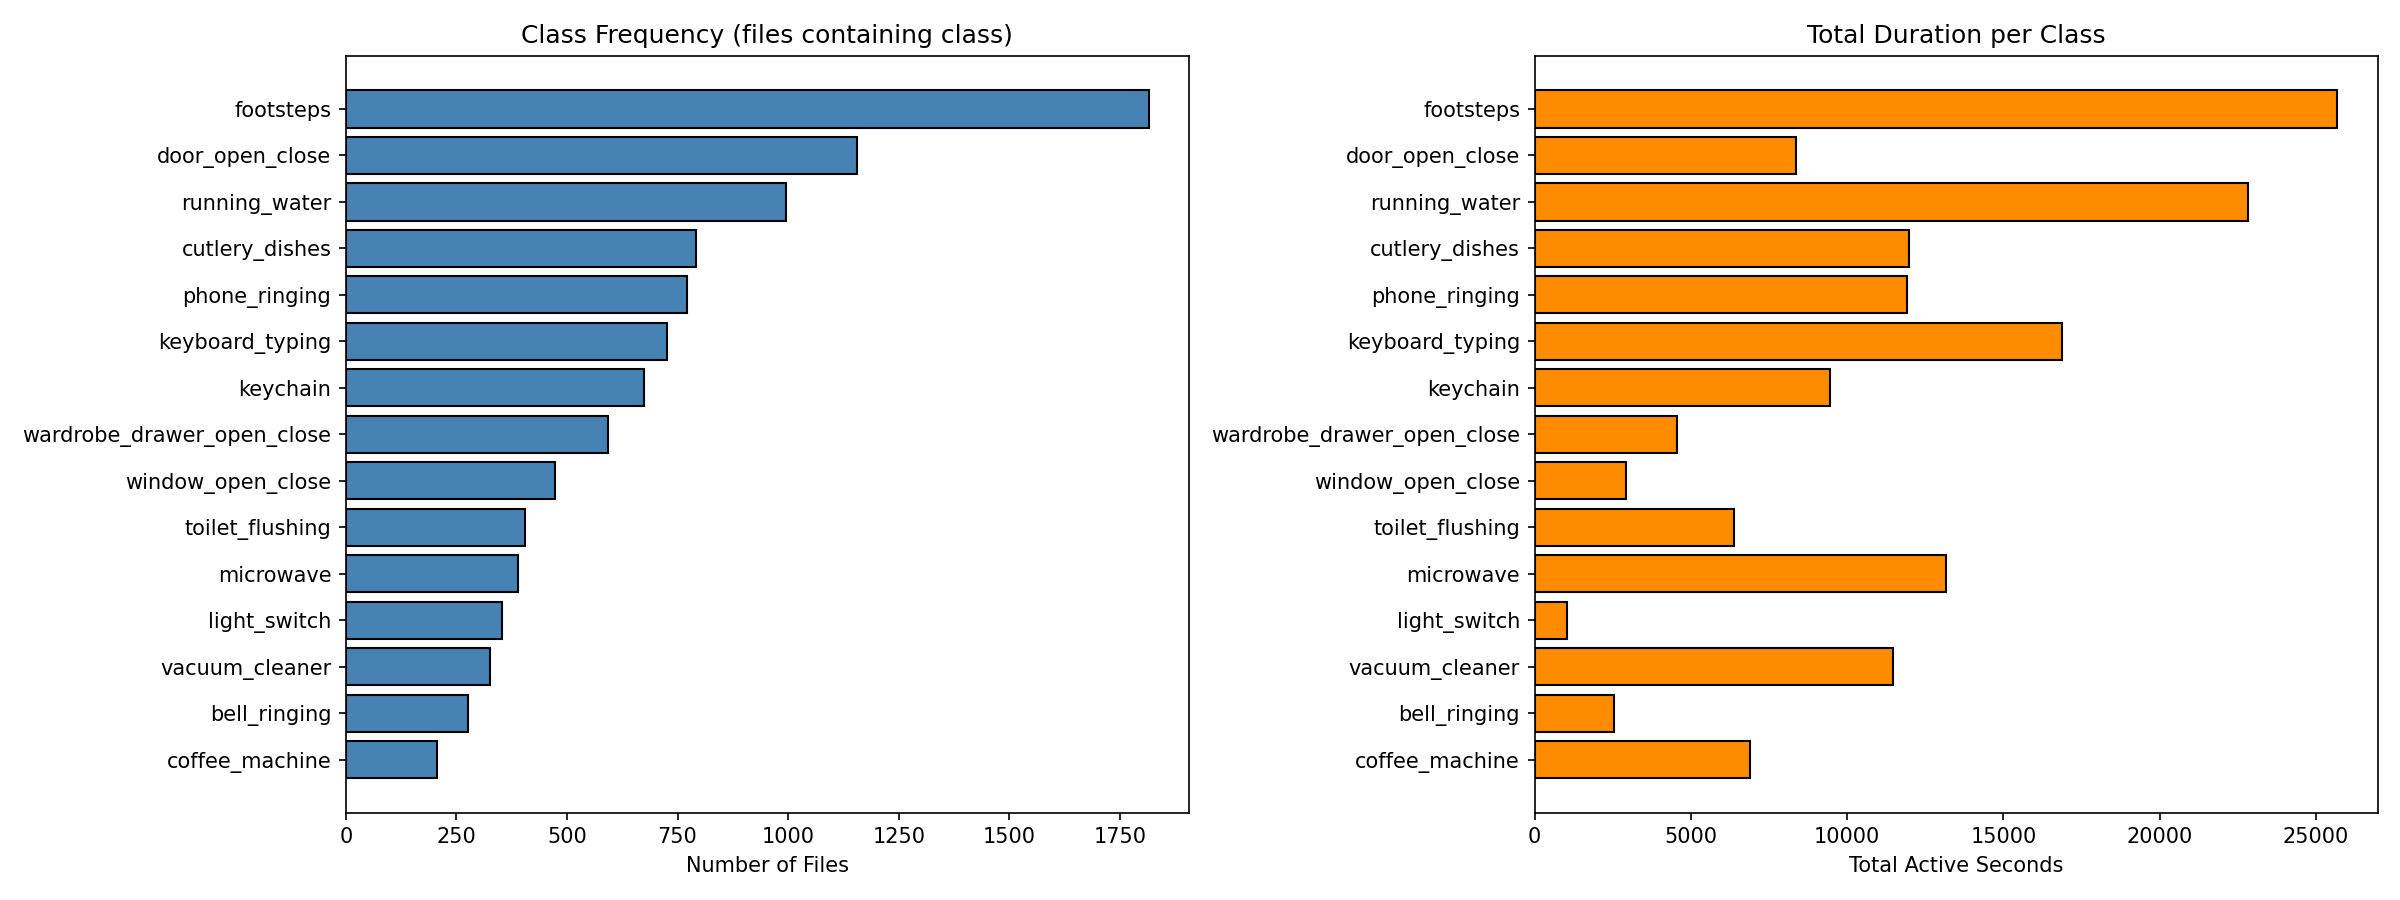
\includegraphics[width=\textwidth]{label_frequency.png}
  \caption{Left: number of files containing each class. Right: total active seconds per class.}
  \label{fig:labelfreq}
\end{figure}
 
\begin{figure}[!h]
  \centering
  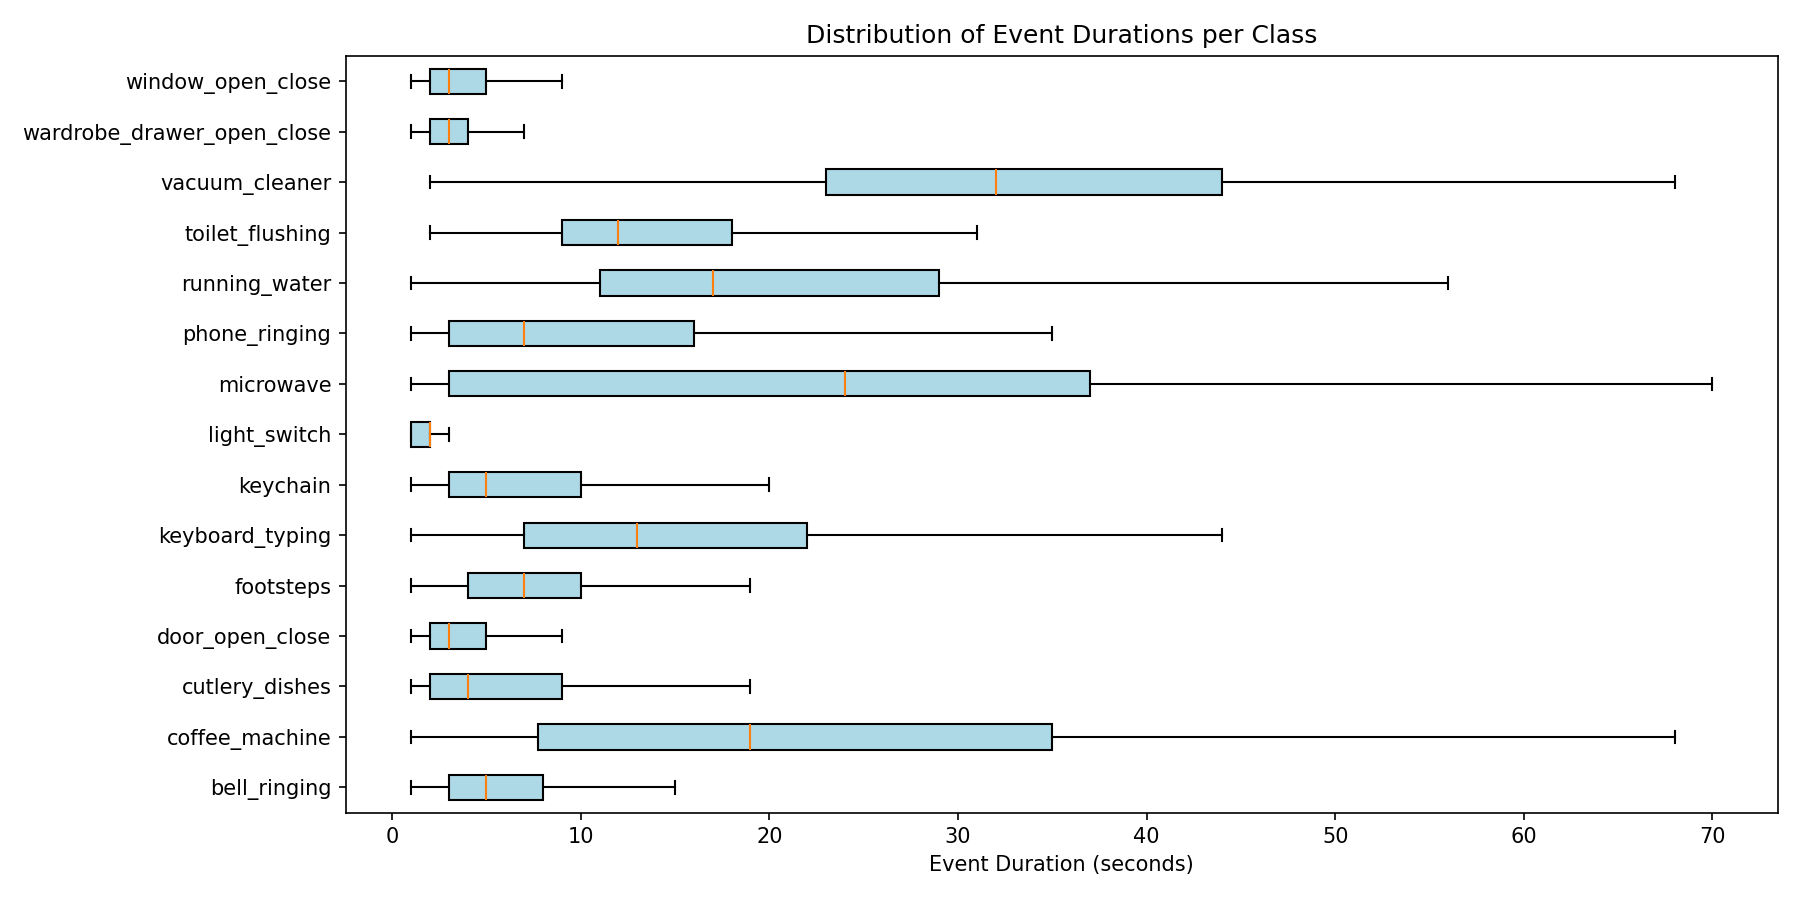
\includegraphics[width=\textwidth]{event_durations.png}
  \caption{Event duration distribution per class (outliers hidden).}
  \label{fig:durations}
\end{figure}
 
\begin{figure}[!h]
  \centering
  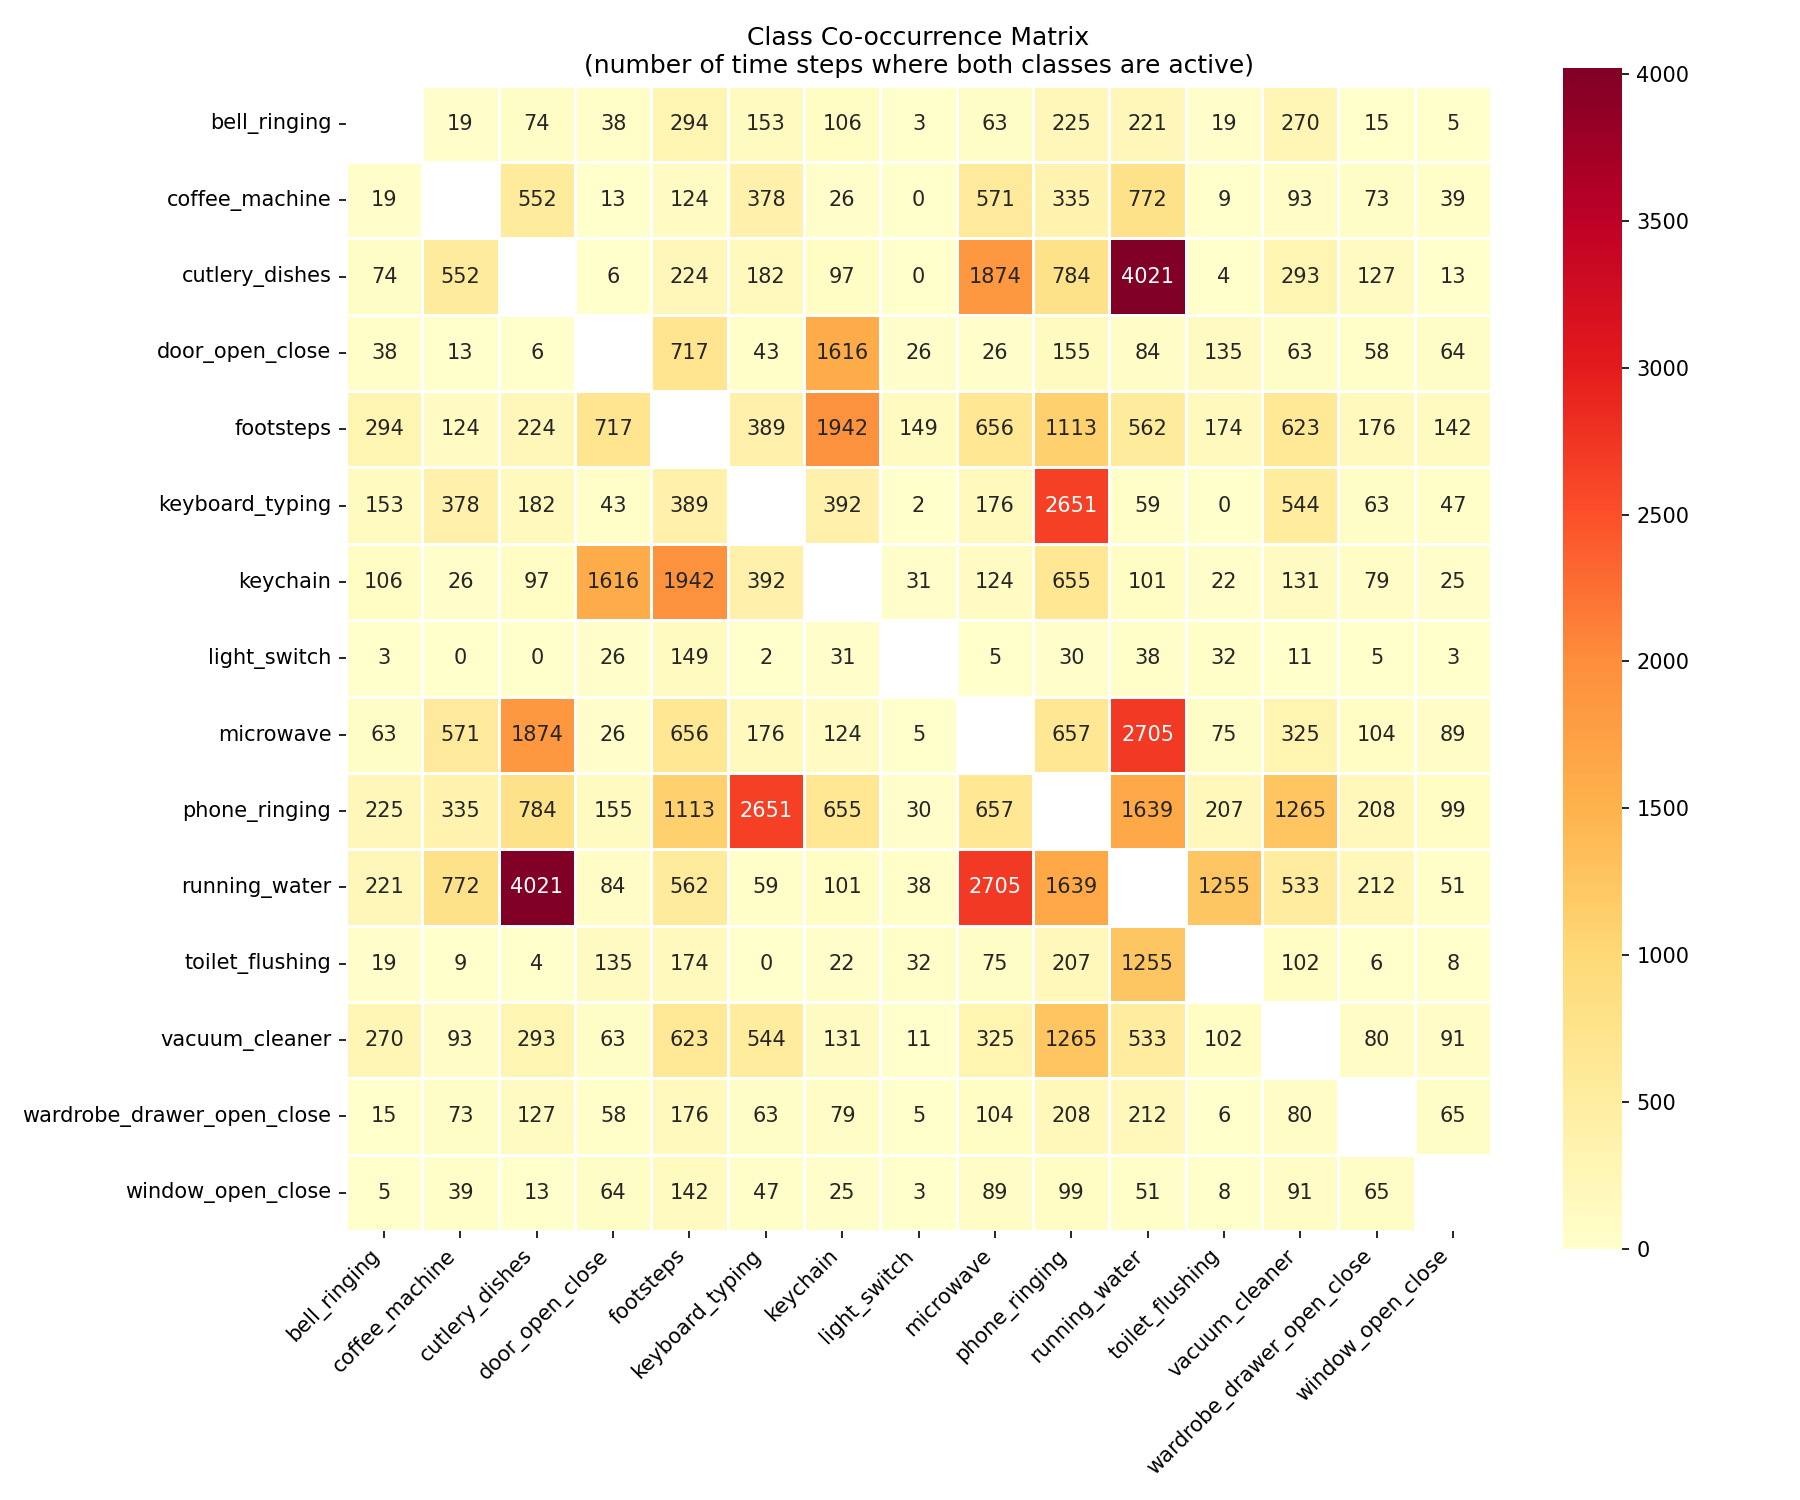
\includegraphics[width=0.85\textwidth]{cooccurrence_matrix.png}
  \caption{Class co-occurrence matrix: number of time steps where both classes are simultaneously active.}
  \label{fig:cooccurrence}
\end{figure}
 
\begin{figure}[!h]
  \centering
  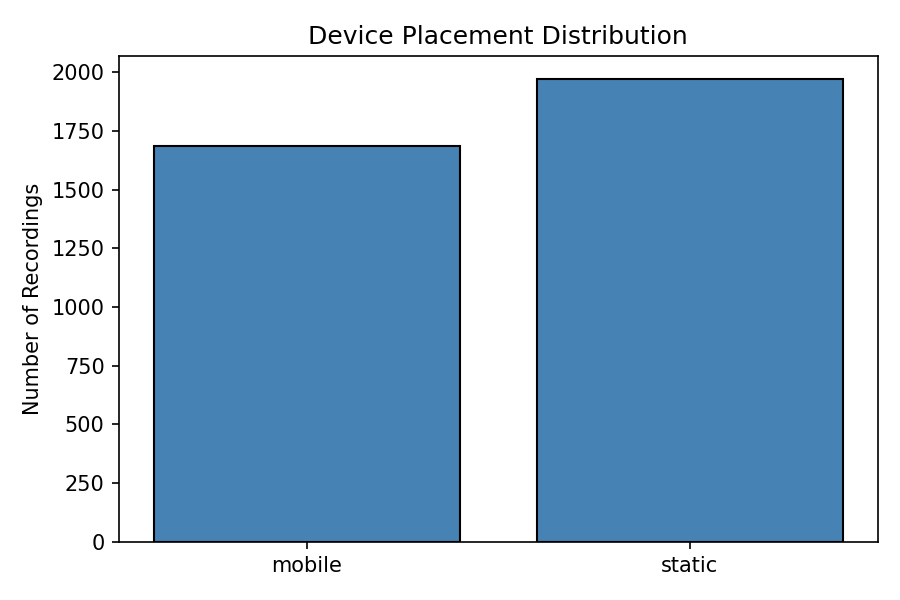
\includegraphics[width=0.5\textwidth]{placement_distribution.png}
  \caption{Distribution of device placement (static vs.\ mobile).}
  \label{fig:placement}
\end{figure}
 
\begin{figure}[!h]
  \centering
  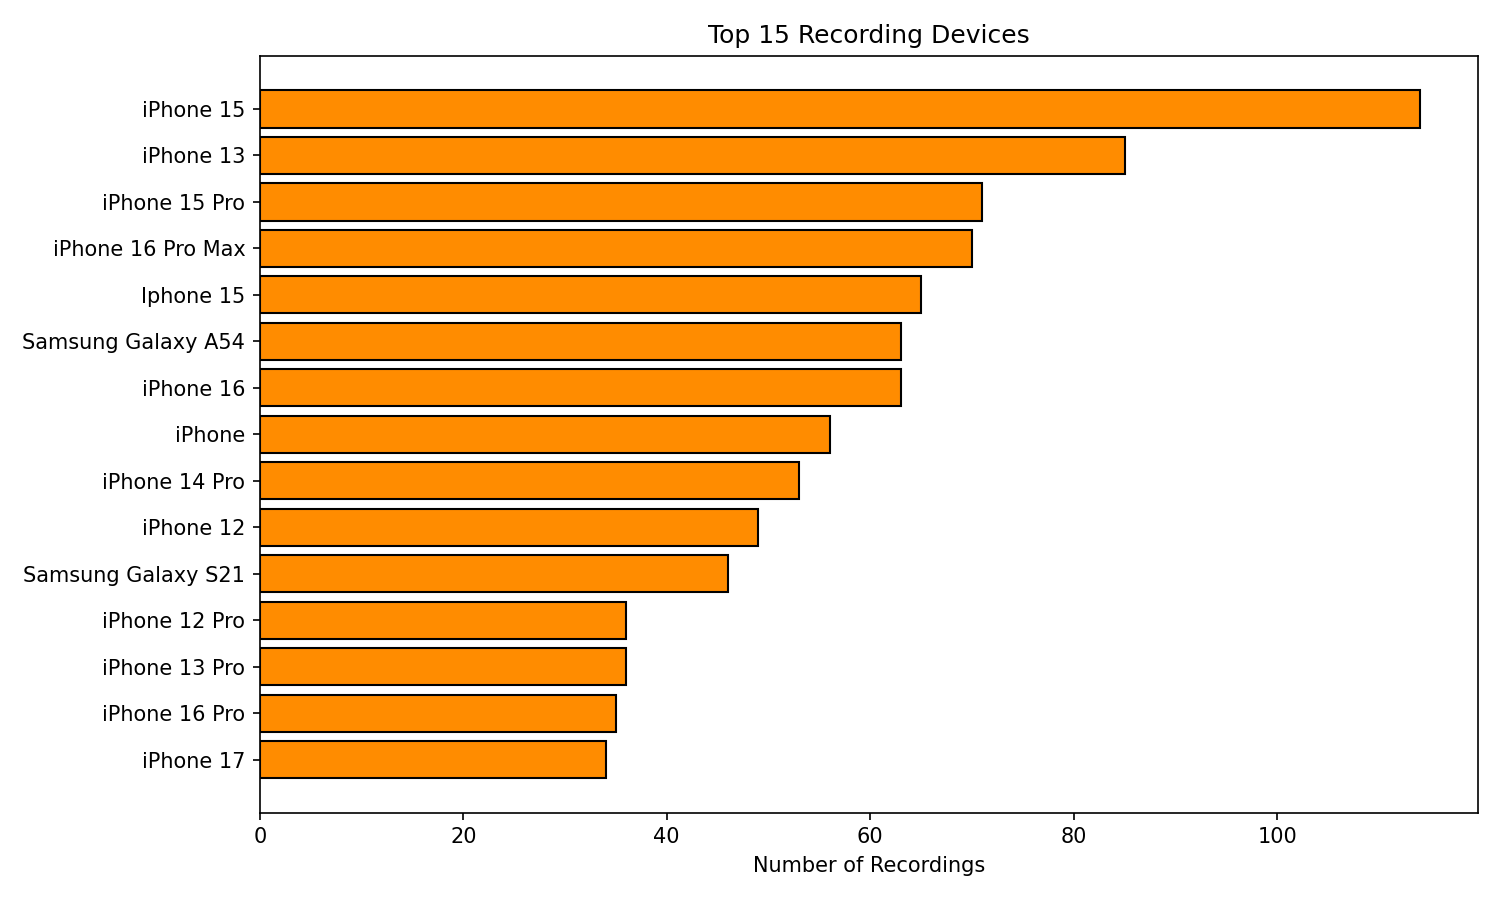
\includegraphics[width=0.85\textwidth]{device_distribution.png}
  \caption{Top 15 recording devices. Iphone and Samsung smartphones dominate the dataset.}
  \label{fig:devices}
\end{figure}
 
\begin{figure}[!h]
  \centering
  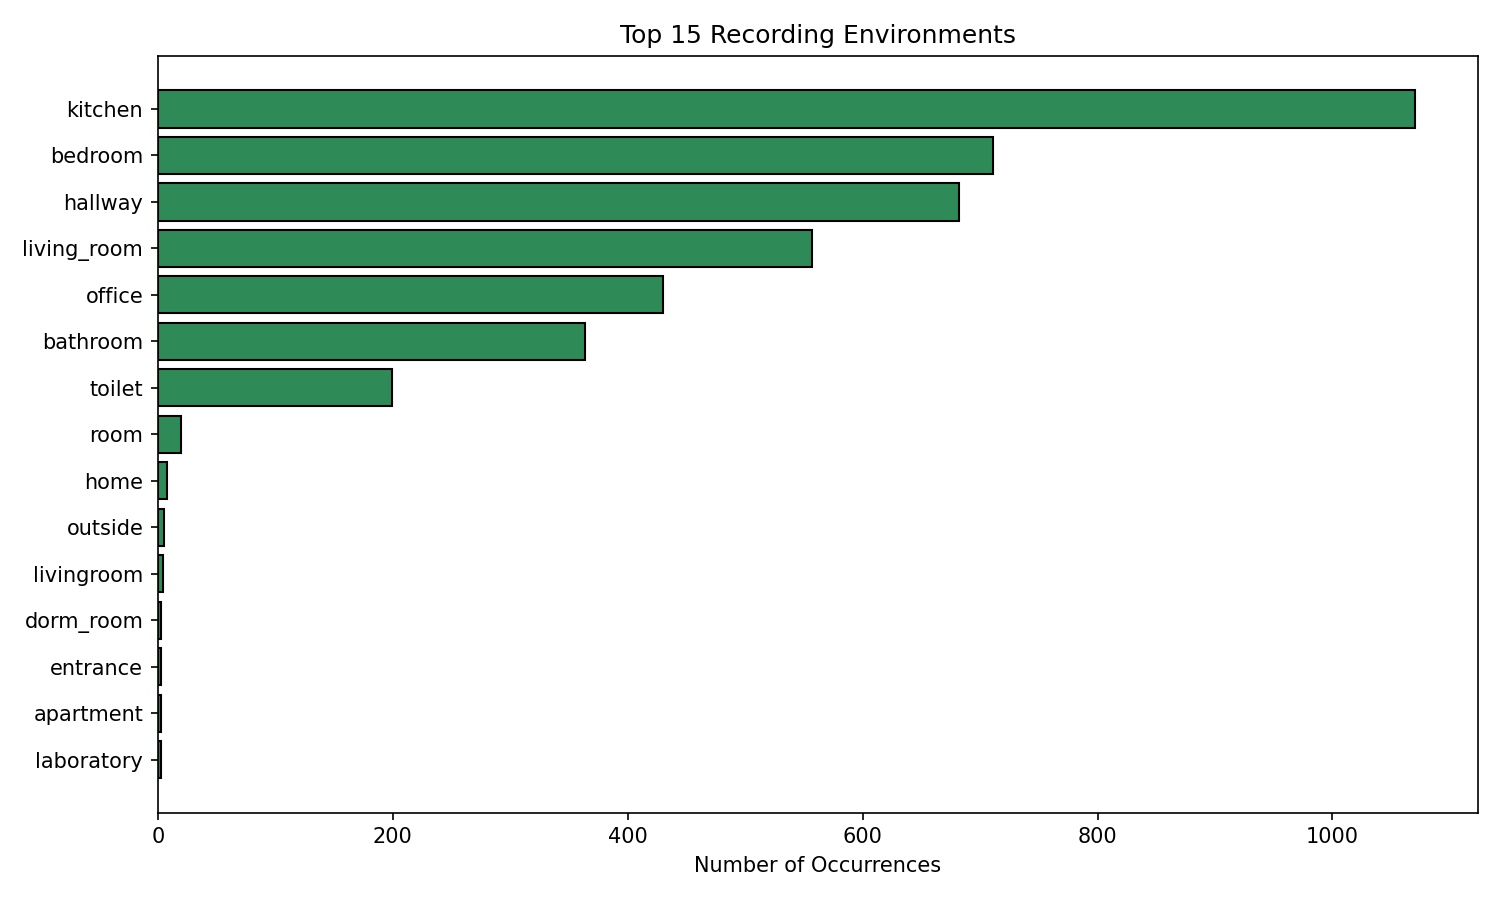
\includegraphics[width=0.85\textwidth]{environment_distribution.png}
  \caption{Top 15 recording environments.}
  \label{fig:environments}
\end{figure}

\begin{figure}[!h]
  \centering
  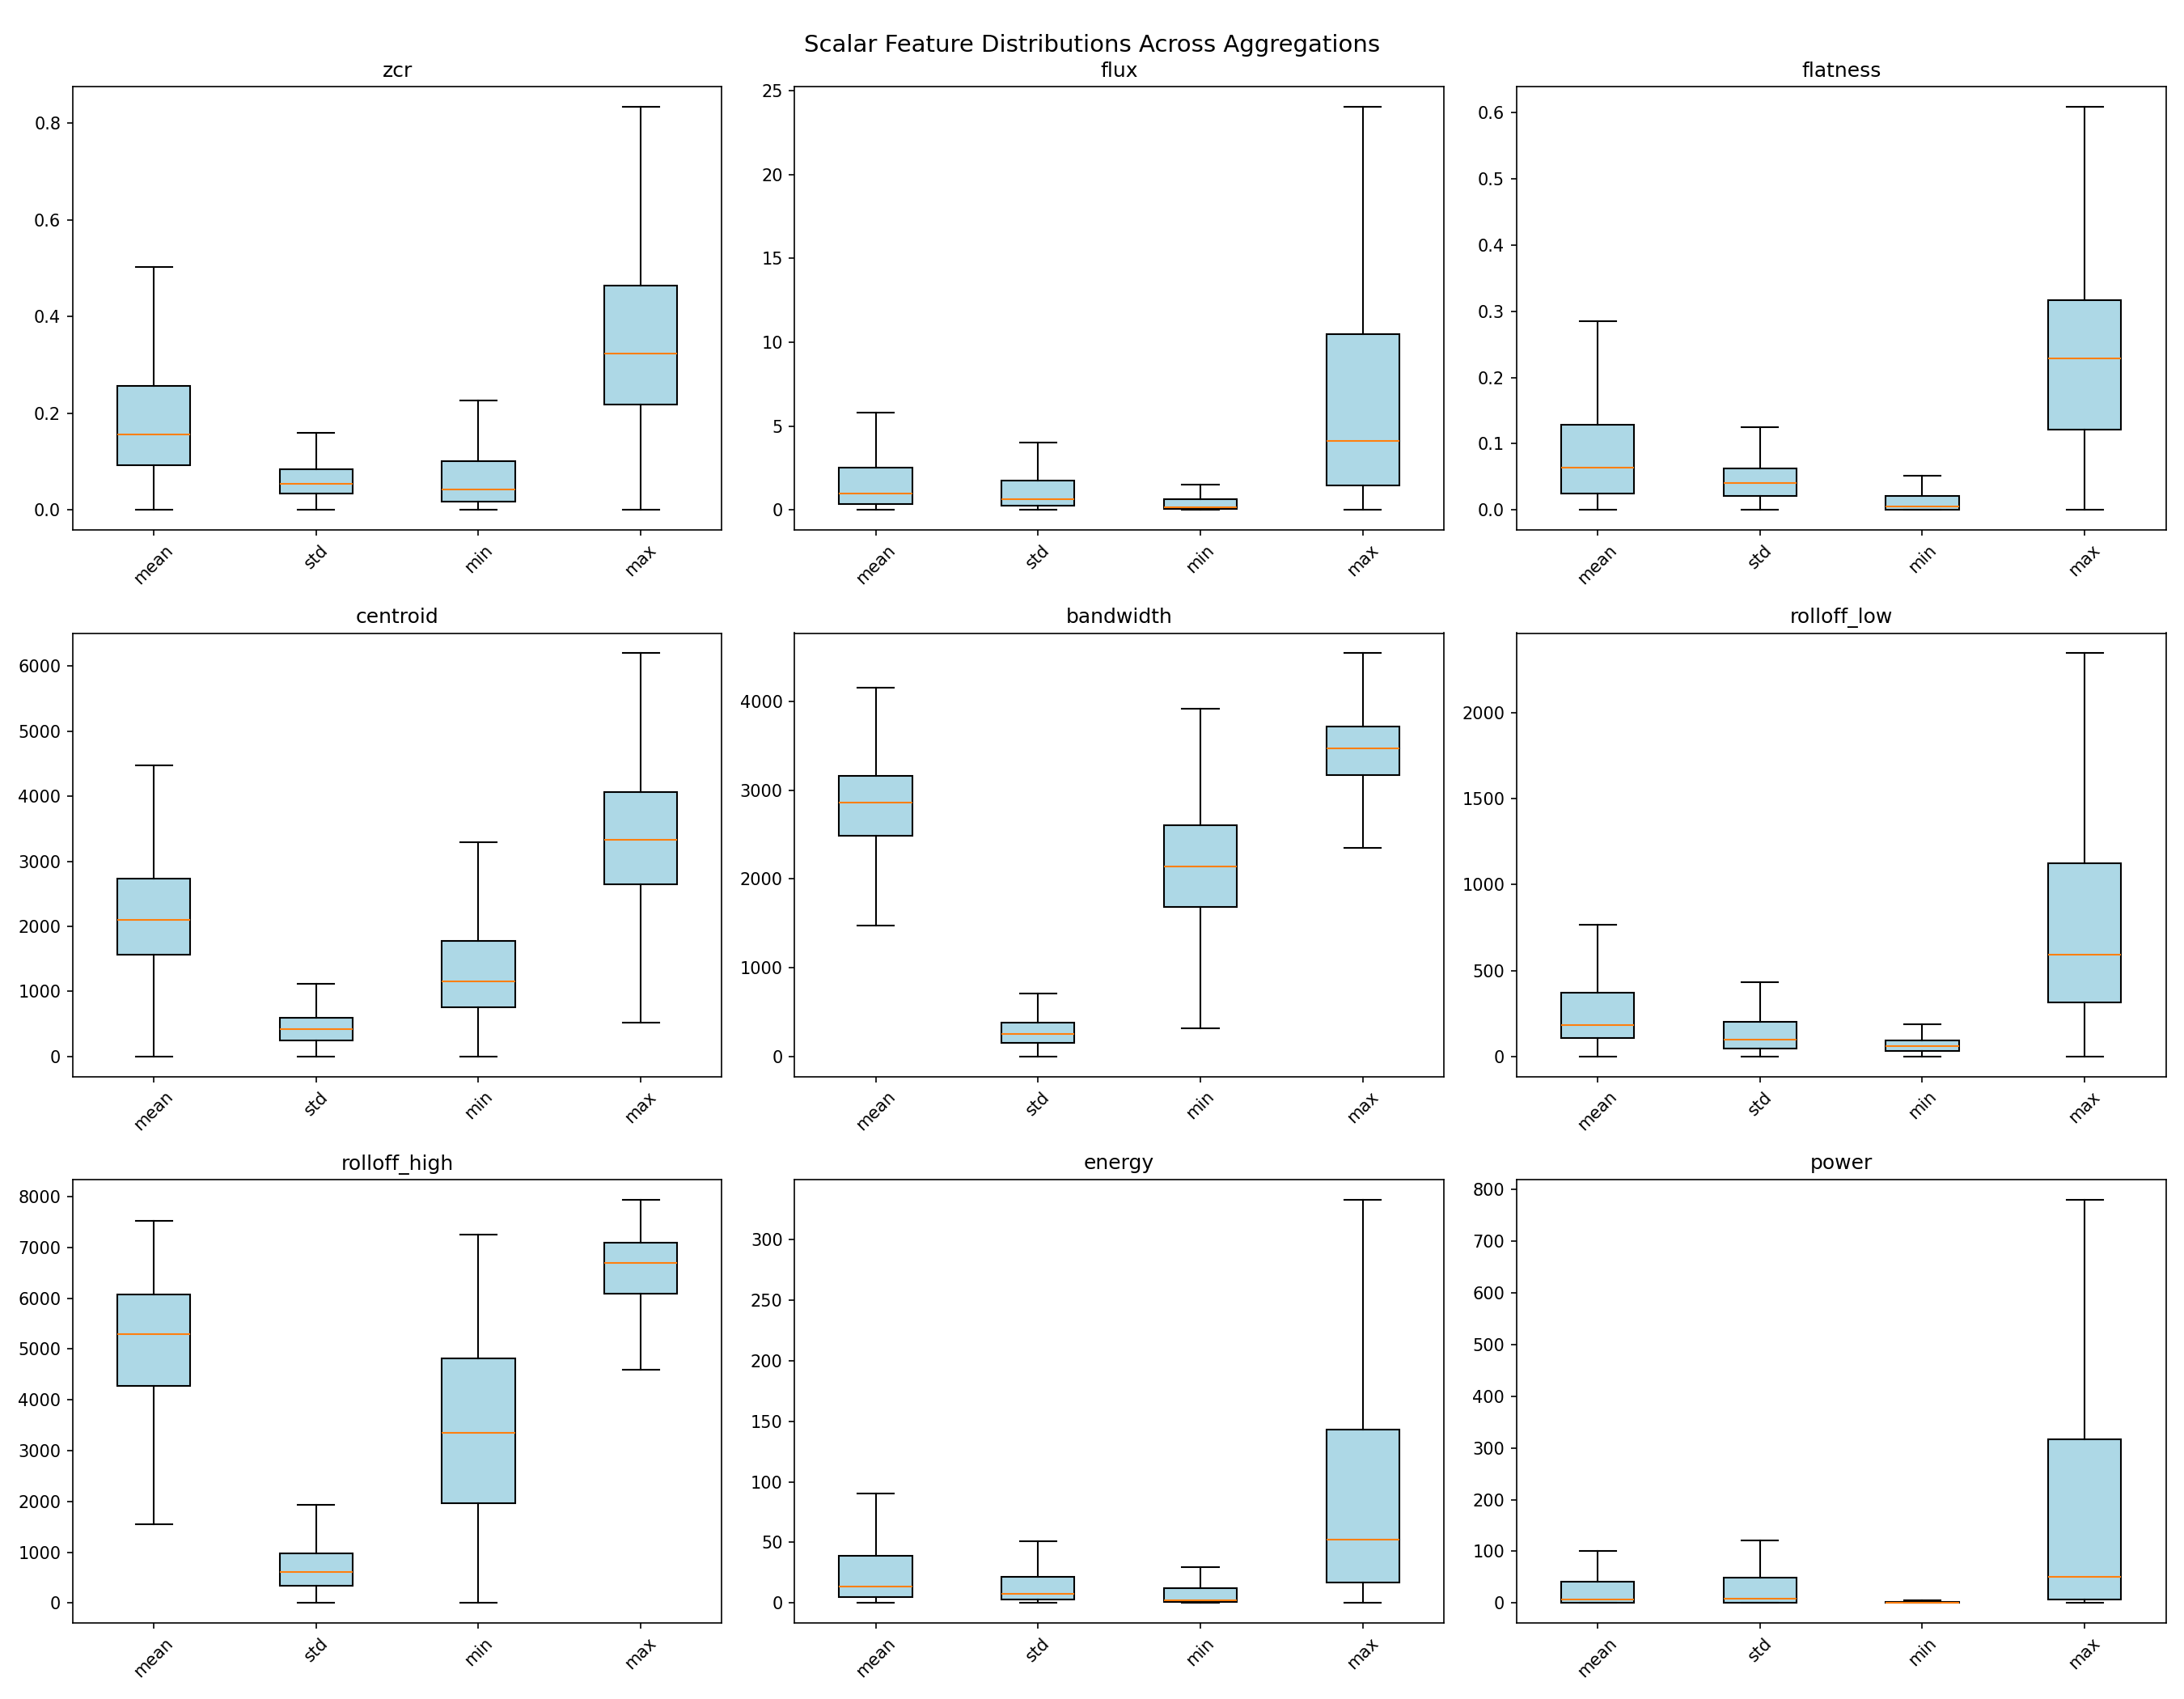
\includegraphics[width=\textwidth]{scalar_feature_boxplots.png}
  \caption{Value distributions for unidimensional features) across the four aggregations. Outliers are hidden for readability.}
  \label{fig:scalarboxplots}
\end{figure}
 
\begin{figure}[!h]
  \centering
  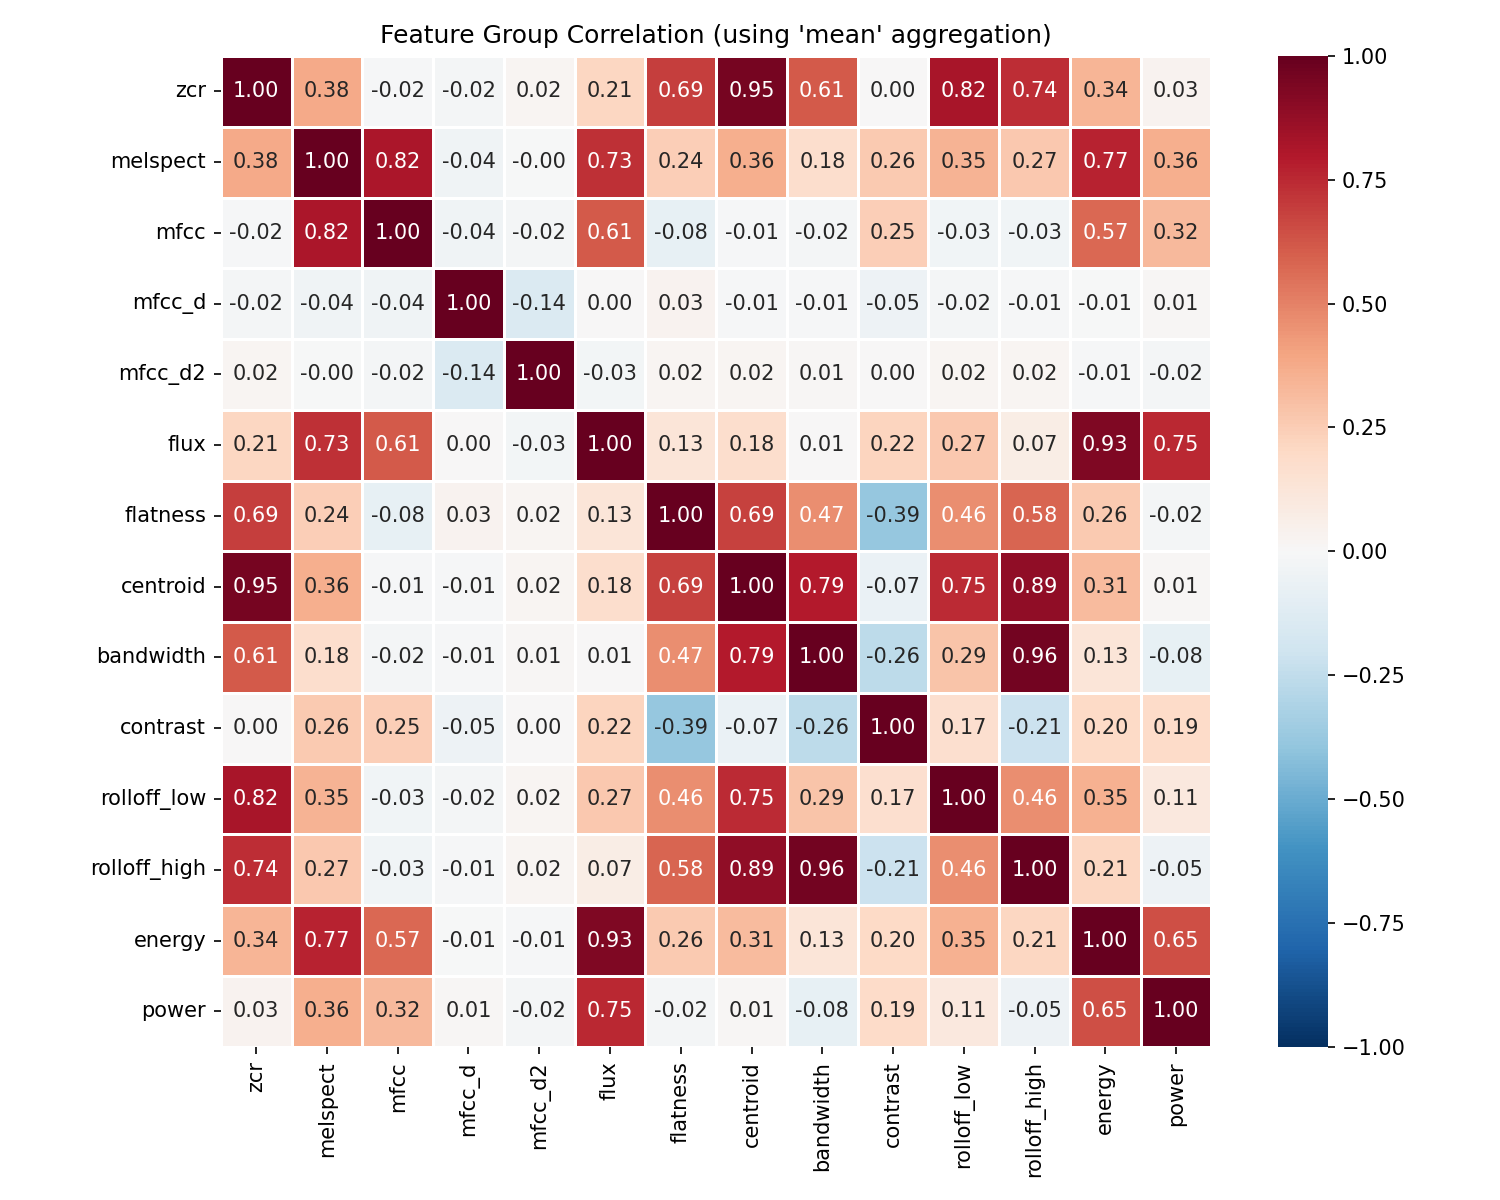
\includegraphics[width=0.85\textwidth]{feature_group_correlation.png}
  \caption{Feature group correlation matrix (mean aggregation).}
  \label{fig:groupcorr}
\end{figure}
 
\begin{figure}[!h]
  \centering
  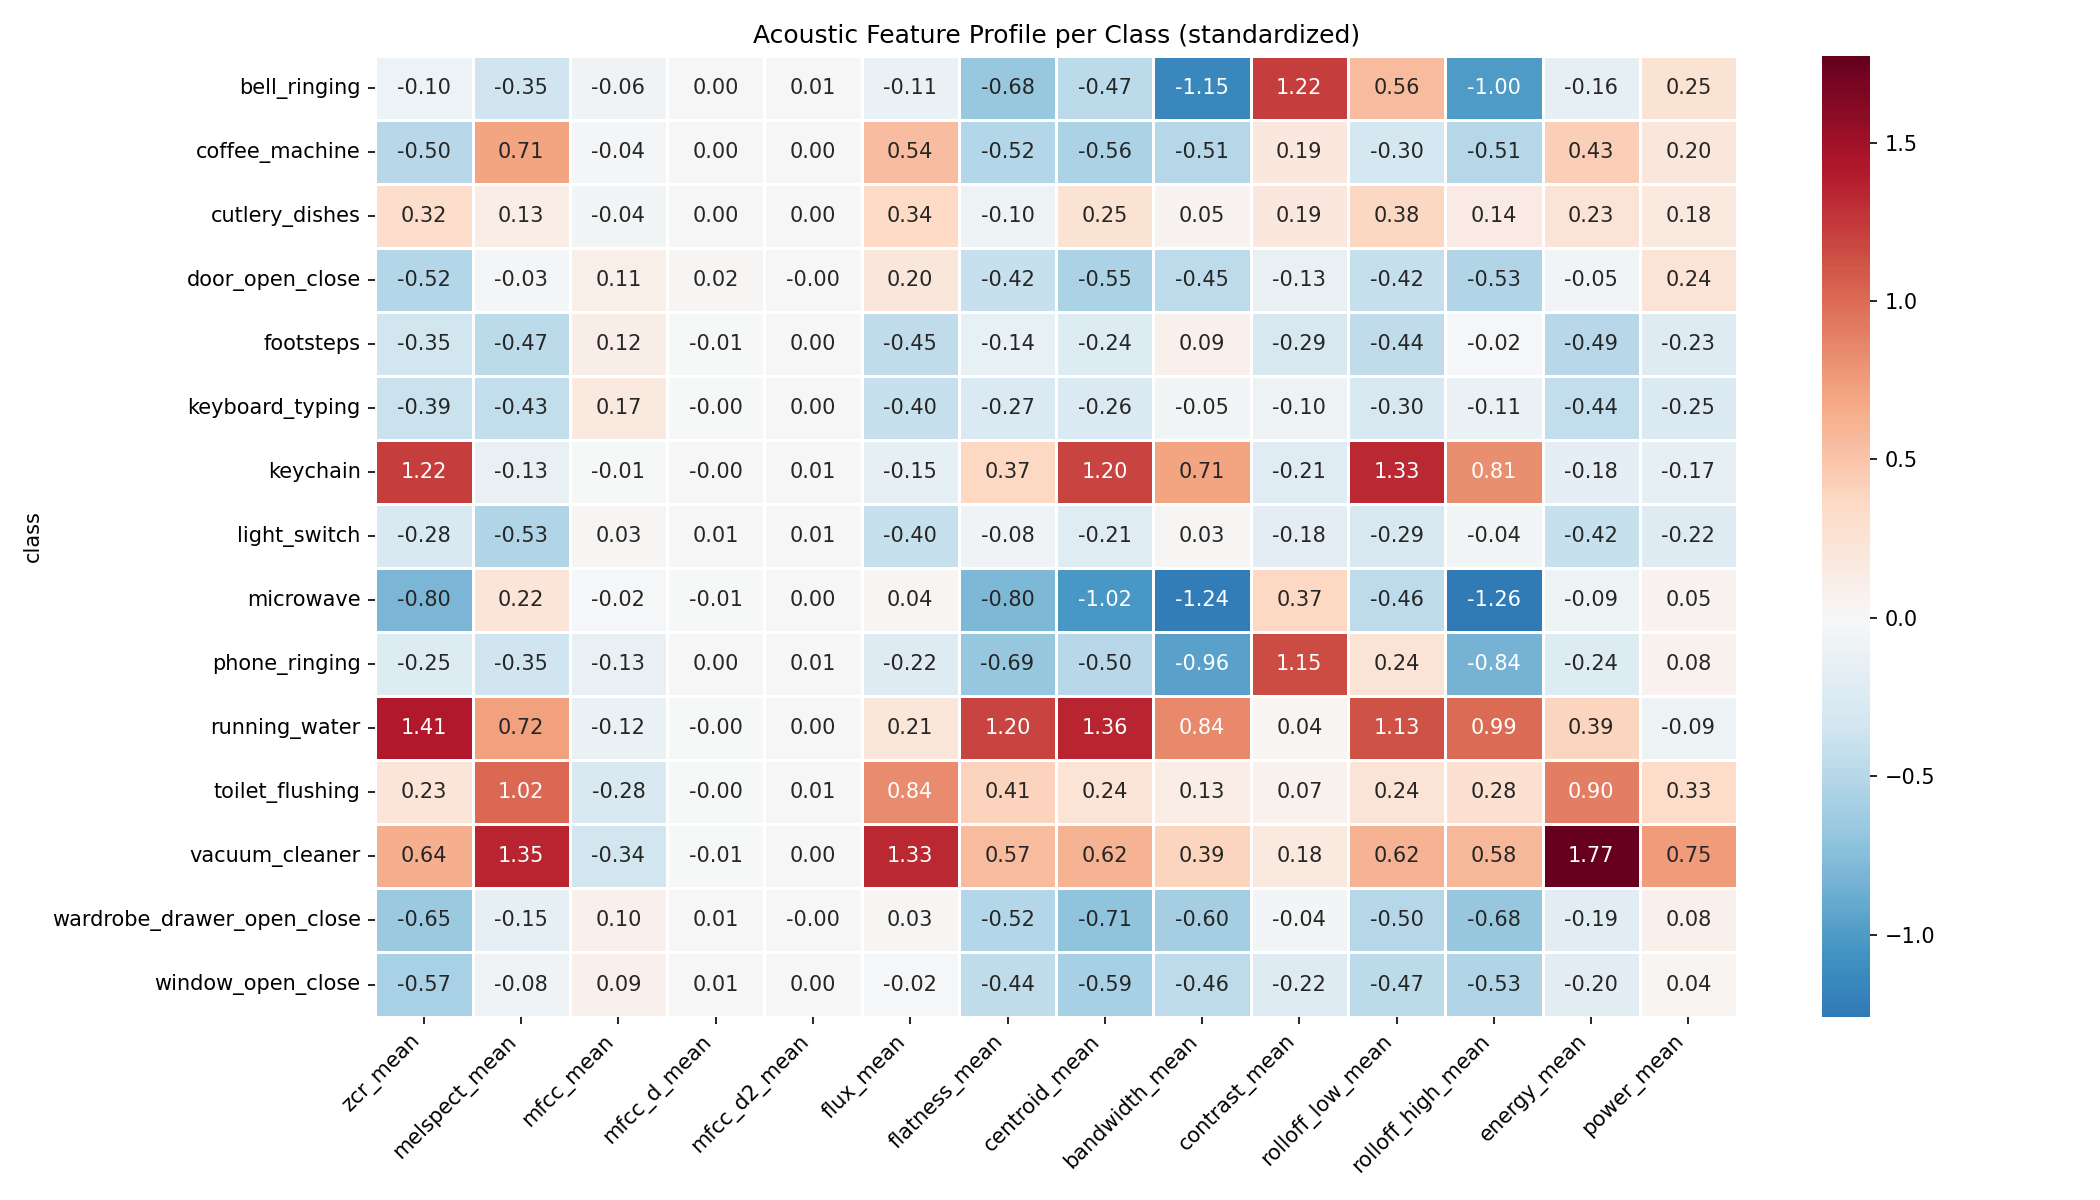
\includegraphics[width=\textwidth]{class_feature_profiles.png}
  \caption{Acoustic feature profile per class (standardized). Each cell shows the mean deviation from the dataset average in standard deviations. Distinctive fingerprints are visible: vacuum cleaner (high energy, melspect), running water (high zcr, flatness), microwave (low centroid, bandwidth).}
  \label{fig:profiles}
\end{figure}
 
\begin{figure}[!h]
  \centering
  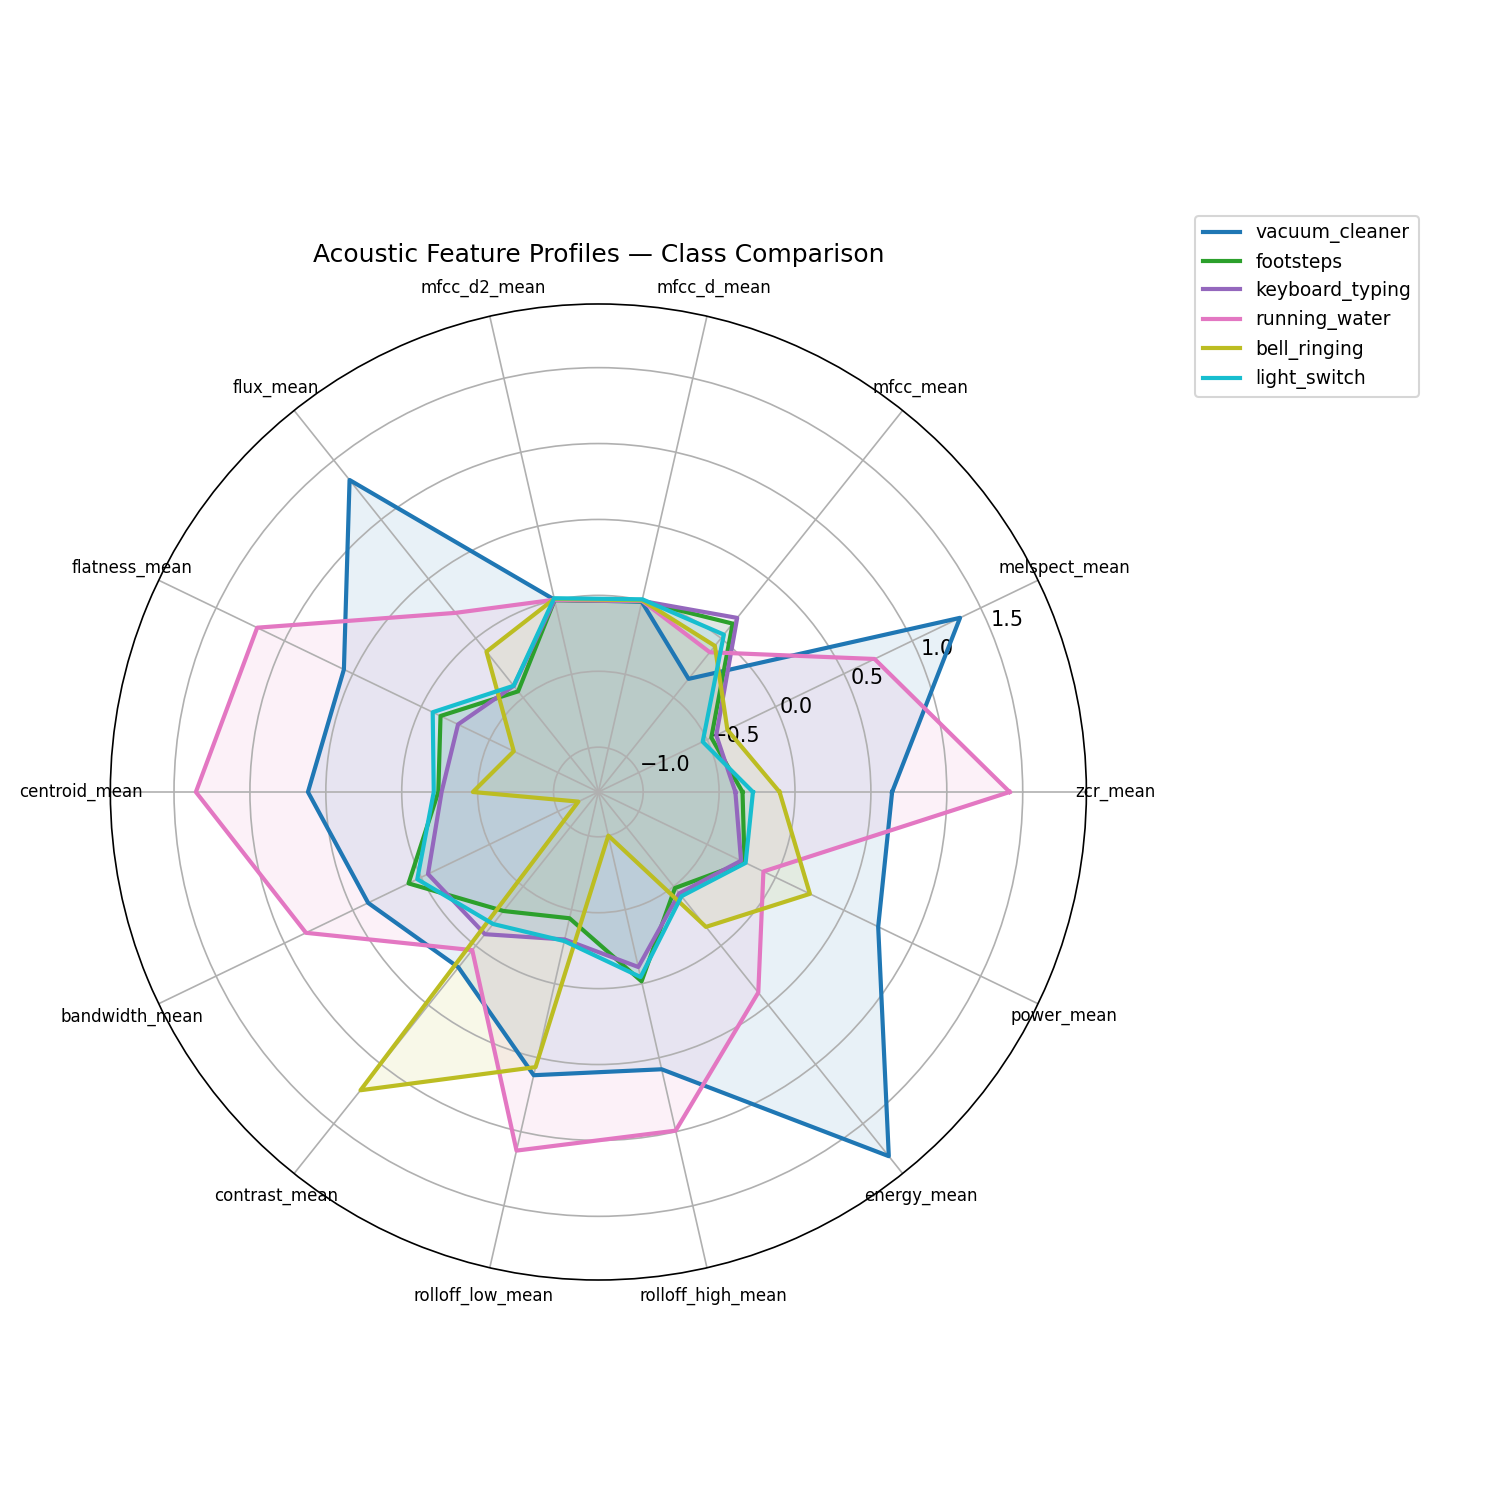
\includegraphics[width=0.85\textwidth]{class_radar_profiles.png}
  \caption{Radar chart comparing acoustic profiles of six selected classes. Each axis represents a mean-aggregated feature.}
  \label{fig:radar}
\end{figure}
 
 
\begin{figure}[!h]
  \centering
  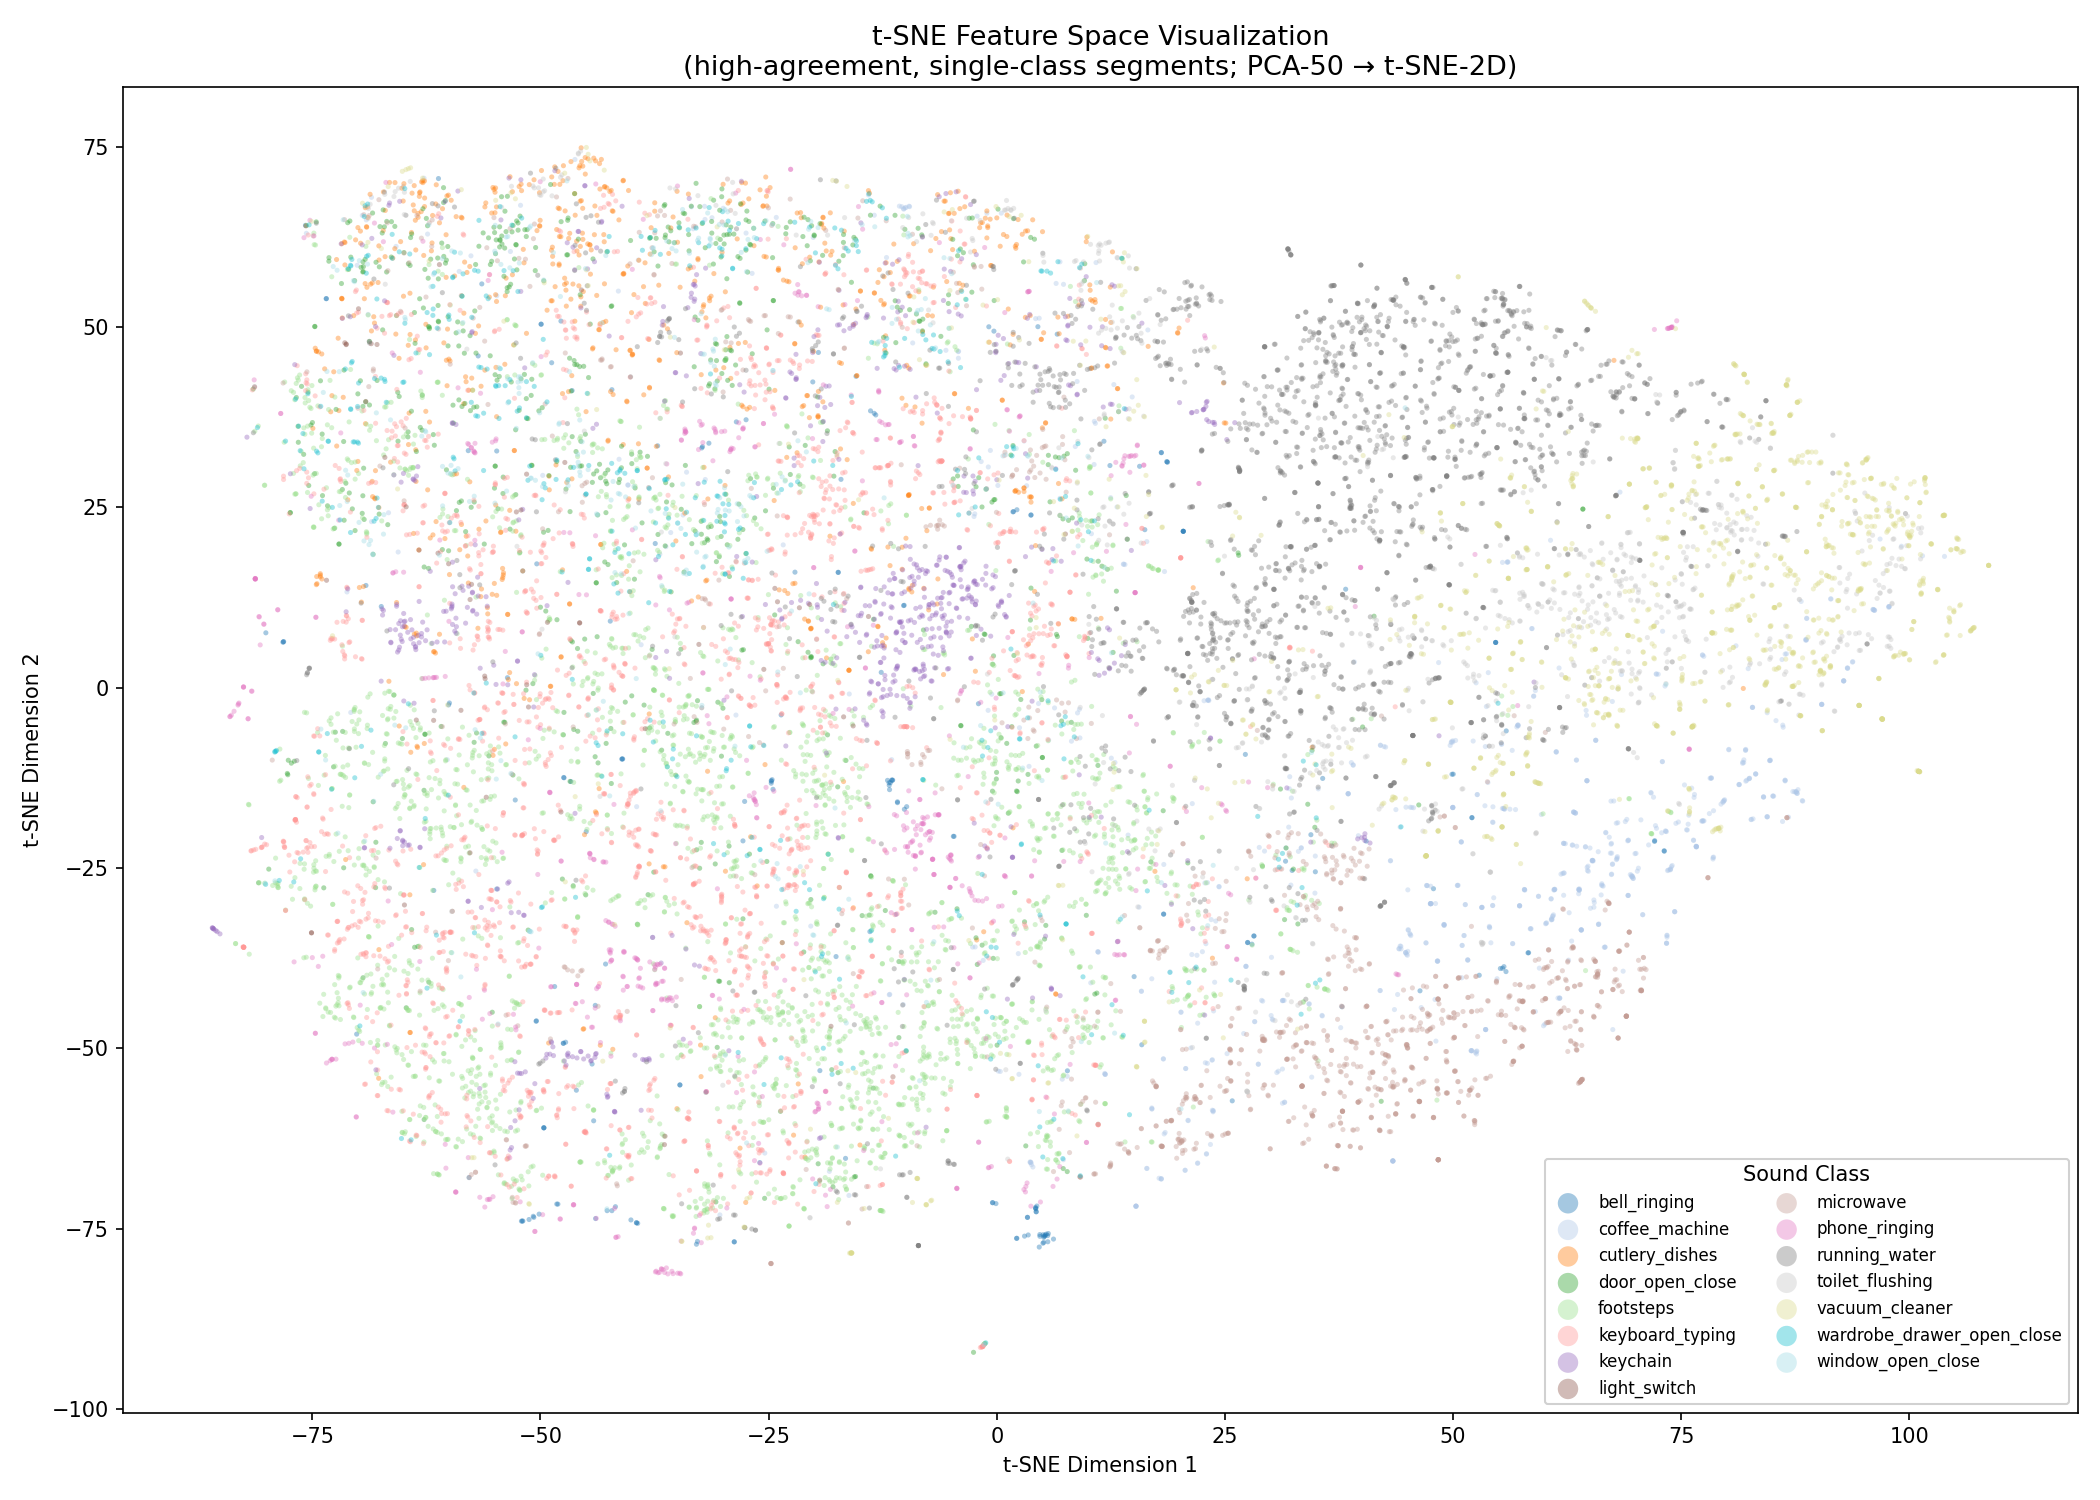
\includegraphics[width=\textwidth]{tsne_feature_space.png}
  \caption{t-SNE visualization of spectral features (PCA-50, perplexity=30). Sustained sounds (vacuum cleaner, running water, microwave) form tight, well separated clusters. Transient events (footsteps, light switch, door) are more diffuse and overlapping.}
  \label{fig:tsne}
\end{figure}

\begin{figure}[!h]
  \centering
  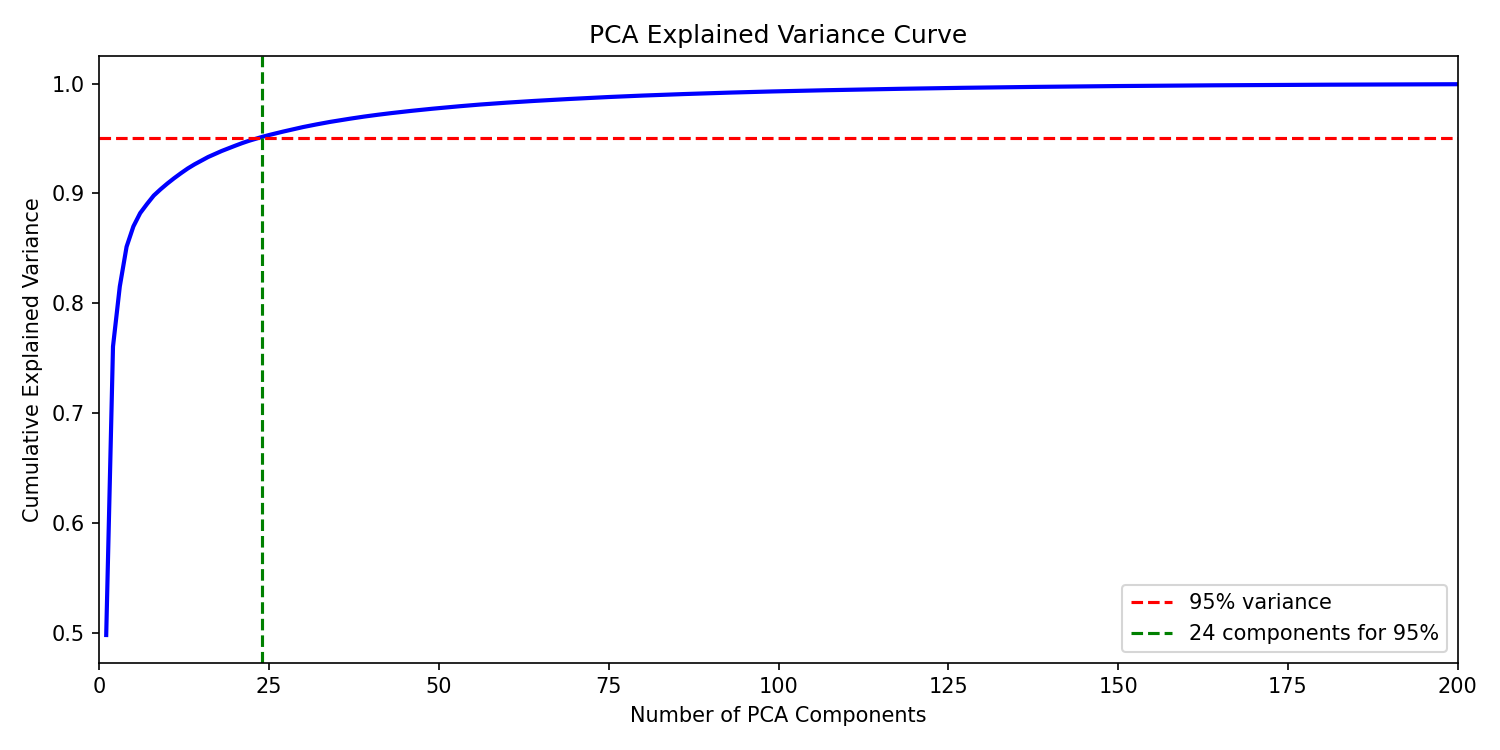
\includegraphics[width=0.85\textwidth]{pca_explained_variance.png}
  \caption{Cumulative PCA explained variance for spectral features (280 dims). 9 components capture 90\%; 24 capture 95\%; 50 capture 97.8\%.}
  \label{fig:pca}
\end{figure}
 
\begin{figure}[!h]
  \centering
  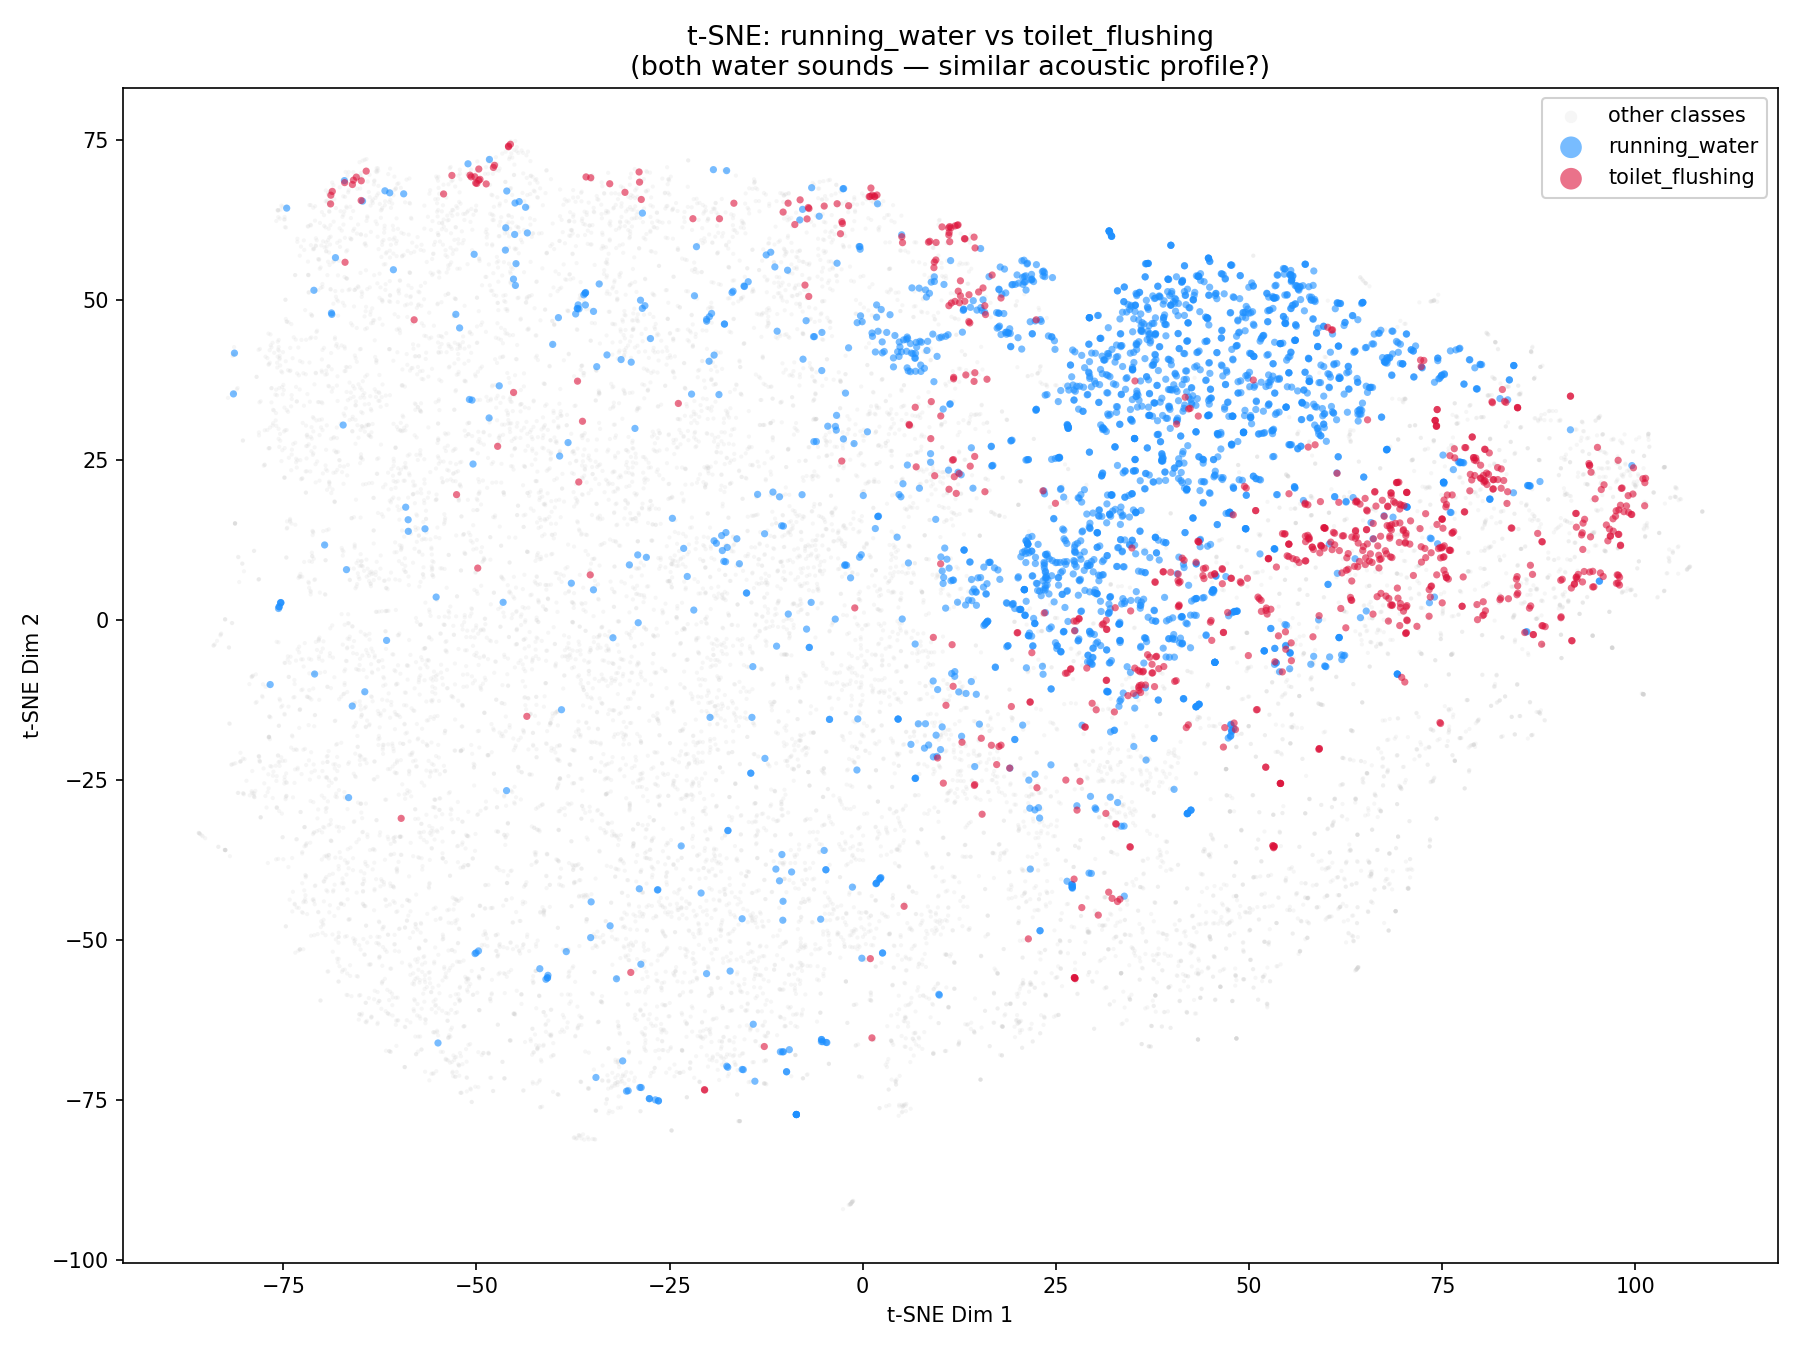
\includegraphics[width=\textwidth]{tsne_pair_water_vs_toilet.png}
  \caption{t-SNE pair highlight: running\_water vs.\ toilet\_flushing.}
  \label{fig:tsnepair1}
\end{figure}
 
\begin{figure}[!h]
  \centering
  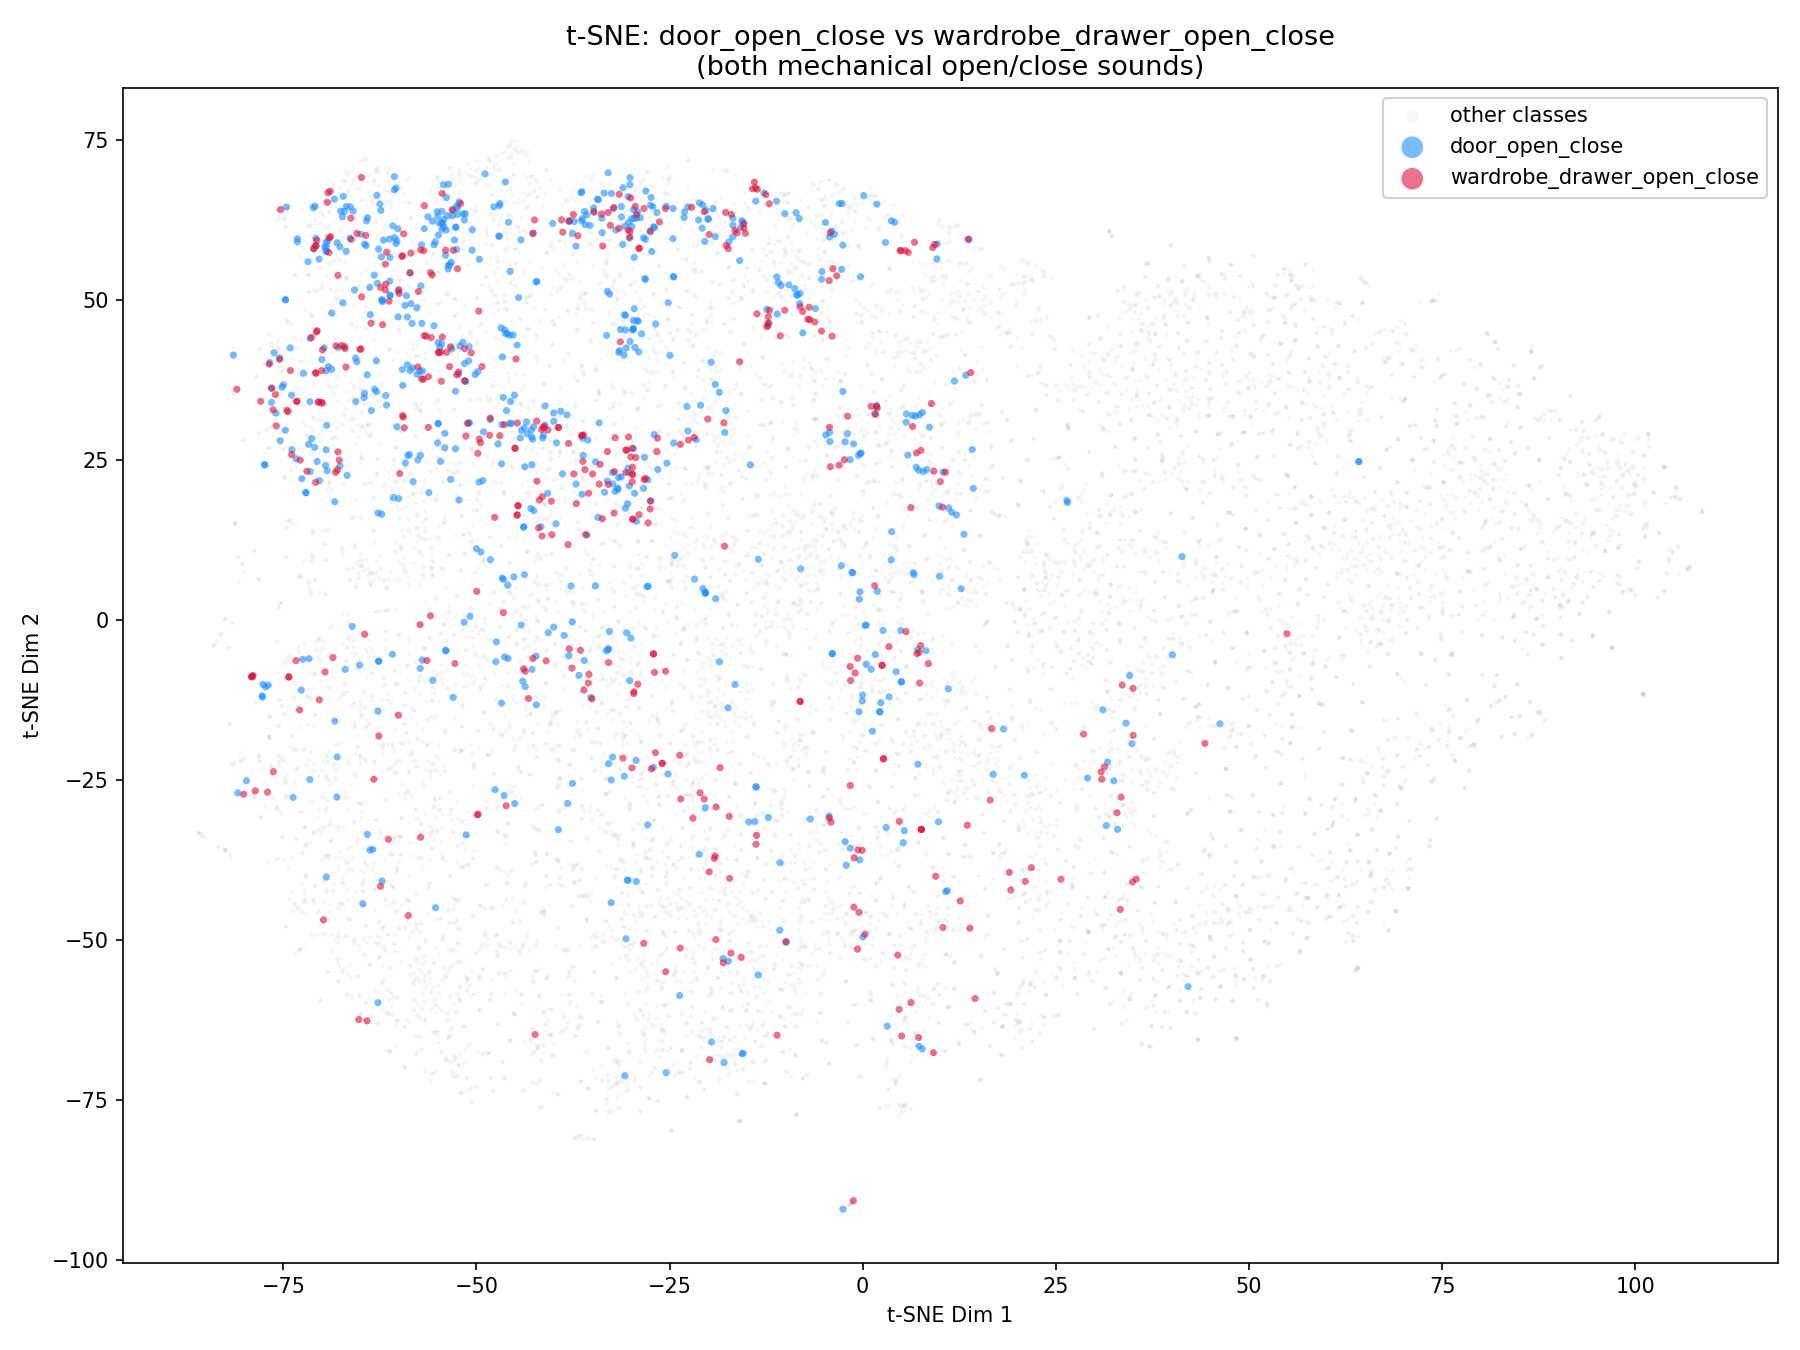
\includegraphics[width=\textwidth]{tsne_pair_door_vs_wardrobe.png}
  \caption{t-SNE pair highlight: door\_open\_close vs.\ wardrobe\_drawer\_open\_close.}
  \label{fig:tsnepair2}
\end{figure}
 
\begin{figure}[!h]
  \centering
  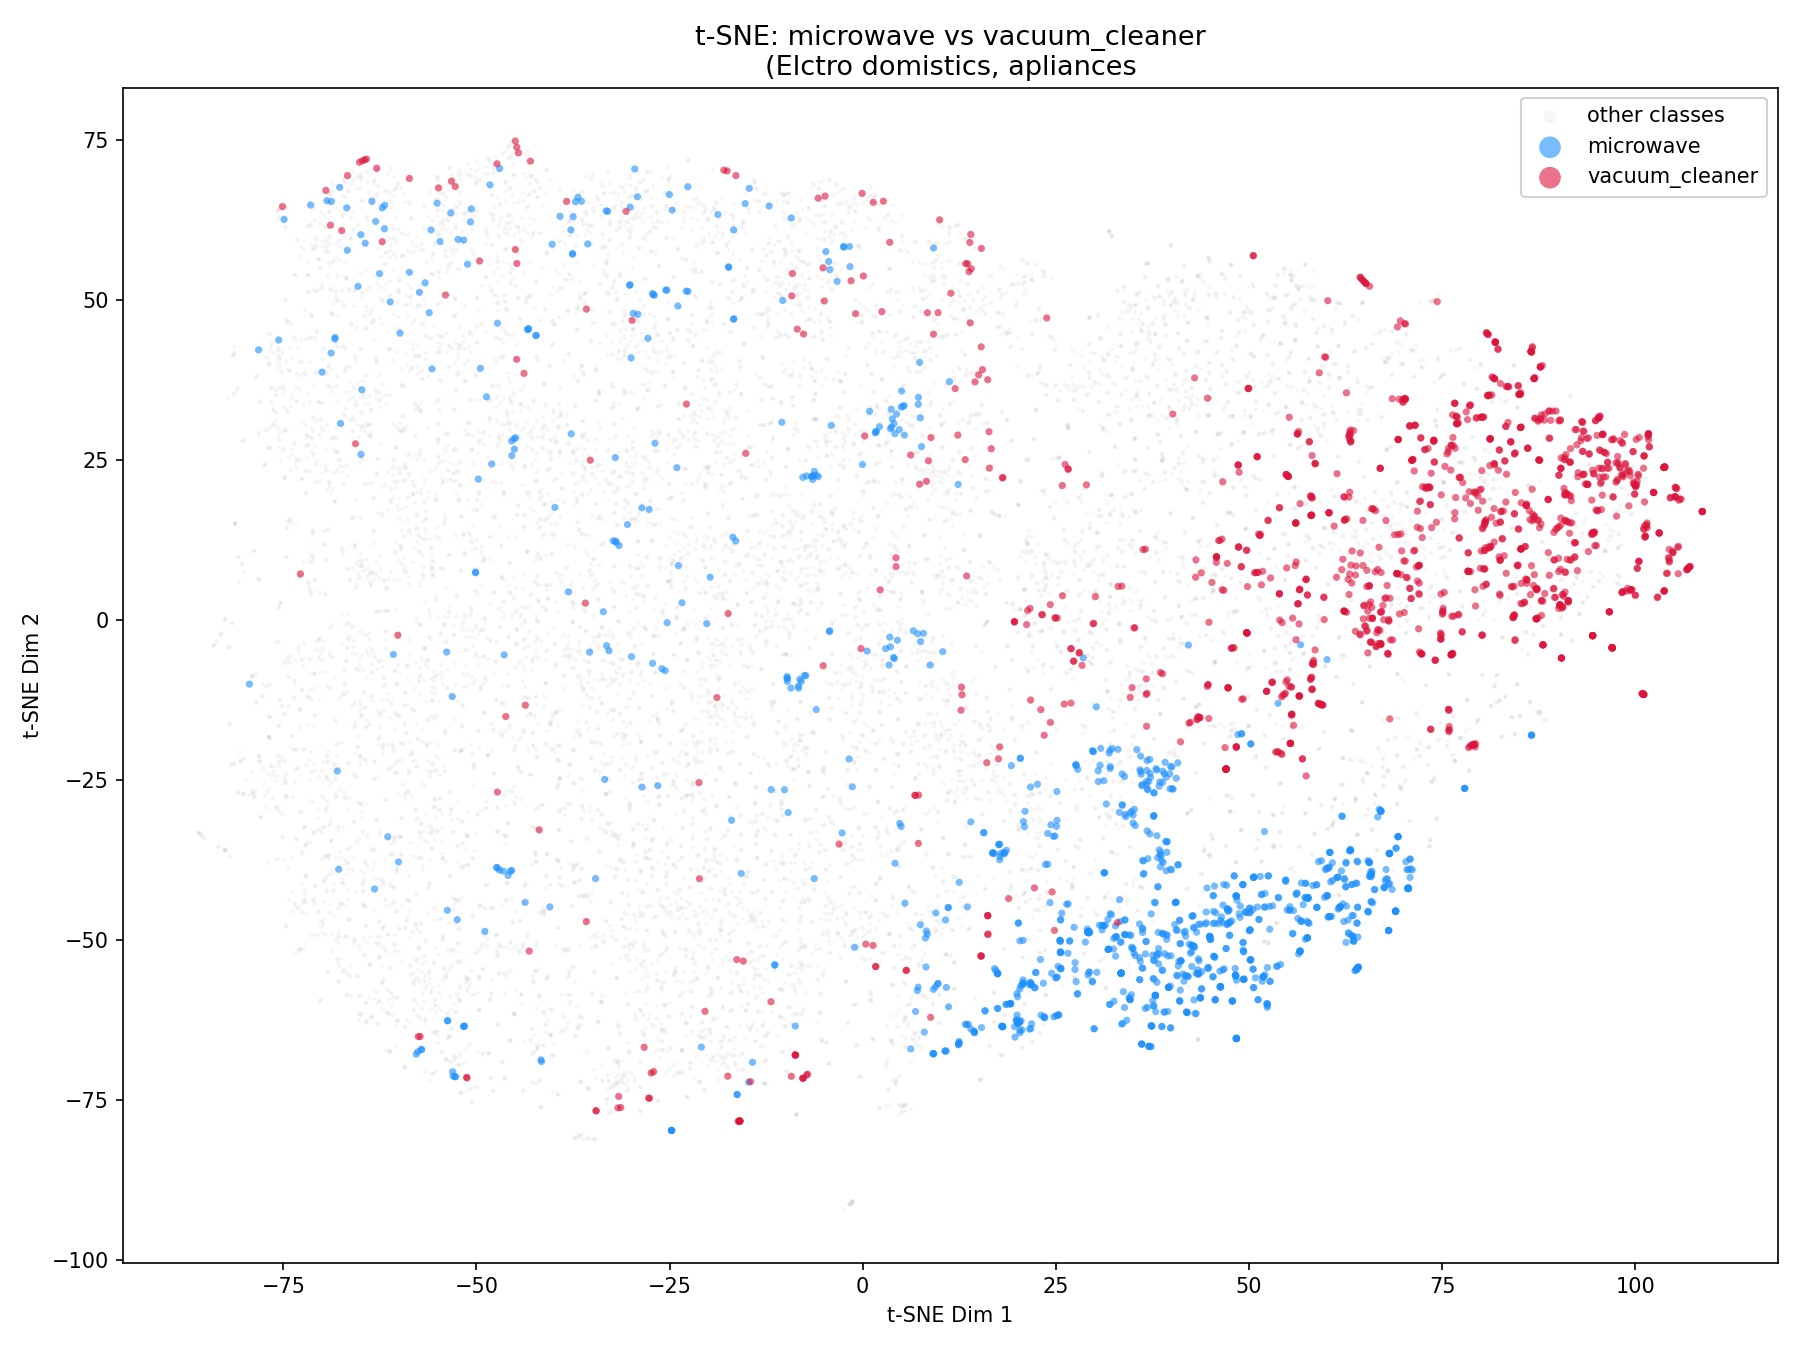
\includegraphics[width=\textwidth]{tsne_pair_vacuum_vs_microwave.png}
  \caption{t-SNE pair highlight: vacuum\_cleaner vs.\ microwave.}
  \label{fig:tsnepair3}
\end{figure}

% Tables
\clearpage
\subsection{Tables}
 
\begin{table}[!h]
  \caption{Label characteristics for all 15 classes, sorted by file count.}
  \label{tab:labels}
  \centering
  \small
  \begin{tabular}{lrrrrr}
    \toprule
    Class & Files & Events & Med.\ dur (s) & Total (s) & \% time \\
    \midrule
    footsteps                   & 1815 & 3063 &  7 & 25683 & 15.3 \\
    door\_open\_close           & 1155 & 1988 &  3 &  8347 &  5.0 \\
    running\_water              &  995 & 1083 & 17 & 22834 & 13.6 \\
    cutlery\_dishes             &  791 & 1681 &  4 & 11976 &  7.1 \\
    phone\_ringing              &  771 & 1109 &  7 & 11926 &  7.1 \\
    keyboard\_typing            &  725 & 1051 & 13 & 16867 & 10.0 \\
    keychain                    &  675 & 1227 &  5 &  9436 &  5.6 \\
    wardrobe\_drawer\_open\_close & 592 & 1184 &  3 &  4568 &  2.7 \\
    window\_open\_close         &  472 &  698 &  3 &  2911 &  1.7 \\
    toilet\_flushing            &  405 &  421 & 12 &  6368 &  3.8 \\
    microwave                   &  390 &  568 & 24 & 13166 &  7.8 \\
    light\_switch               &  354 &  430 &  2 &  1046 &  0.6 \\
    vacuum\_cleaner             &  325 &  340 & 32 & 11452 &  6.8 \\
    bell\_ringing               &  276 &  349 &  5 &  2541 &  1.5 \\
    coffee\_machine             &  207 &  304 & 19 &  6898 &  4.1 \\
    \bottomrule
  \end{tabular}
\end{table}
 
 
\begin{table}[!h]
  \caption{Most frequent sound events per recording environment (top environments)}
  \label{tab:envevents}
  \centering
  \small
  \begin{tabular}{llll}
    \toprule
    Environment & Top 1 class & Top 2 class & Top 3 class \\
    \midrule
    kitchen      & running\_water     & cutlery\_dishes   & footsteps \\
    living room  & footsteps          & door\_open\_close  & keyboard\_typing \\
    office       & keyboard\_typing   & phone\_ringing     & footsteps \\
    bathroom     & toilet\_flushing   & running\_water     & footsteps \\
    bedroom      & footsteps          & door\_open\_close  & wardrobe\_d.\_o.\_c. \\
    hallway      & footsteps          & door\_open\_close  & keychain \\
    \bottomrule
  \end{tabular}
\end{table}
 
% ============================================================
% 3. AUDIO FEATURES — STATISTICS
% ============================================================
 
\begin{table}[!h]
  \caption{Feature statistics per feature group (raw, before normalization)}
  \label{tab:featstats}
  \centering
  \small
  \begin{tabular}{lrrrrr}
    \toprule
    Feature group & Dims & Mean & Std & Min & Max \\
    \midrule
    zcr           &   4 & 0.17    & 0.17     & 0.0   & 0.94 \\
    melspect      & 512 & 3.67    & 2.67     & 0.0   & 13.18 \\
    mfcc          & 128 & $-$1.23 & 12.38    & $-$130.3 & 44.91 \\
    mfcc\_d       & 128 & 0.05    & 0.47     & $-$15.4 & 17.21 \\
    mfcc\_d2      & 128 & 0.03    & 0.30     & $-$9.8  & 8.82 \\
    flux          &   4 & 3.19    & 6.87     & 0.0   & 166.60 \\
    flatness      &   4 & 0.10    & 0.12     & 0.0   & 1.00 \\
    centroid      &   4 & 1841.80 & 1349.48  & 0.0   & 7615.98 \\
    bandwidth     &   4 & 2149.69 & 1265.24  & 0.0   & 4951.66 \\
    contrast      &  28 & 13.83   & 12.99    & 0.0   & 80.11 \\
    rolloff\_low  &   4 & 353.11  & 540.03   & 0.0   & 7437.50 \\
    rolloff\_high &   4 & 3900.31 & 2470.89  & 0.0   & 7937.50 \\
    energy        &   4 & 44.90   & 91.70    & 0.0   & 1978.07 \\
    power         &   4 & 179.04  & 828.71   & 0.0   & 67940.88 \\
    \bottomrule
  \end{tabular}
\end{table}
 


\clearpage
\section{Disclosure of LLM and AI Tool Use}
% This section is mandatory [cite: 1463-1469].
\begin{itemize}
    \item \textbf{Tools Used:} Yes, we used different LLM such as Claude and DeepSeek.
    \item \textbf{Tasks:} The tools were used for code improvement, debugging, and generating fancy plots. Also used for brainstorming, concepts simplification, rephrasing, organizing ideas, improving clarity of technical descriptions and grammatical and orthographical checks. 
All generated code was executed on our dataset, outputs were manually verified against expected behavior, and all results reported in this document were produced by running the verified code on the actual dataset. 
Interpretations and conclusions were written by the authors based on the observed results and outputs of the implemented codes.
\end{itemize}



\end{document}